\chapter{Results}\label{chap:results}

This chapter outlines the results of this research.
%
% produced in the process of implementing the
% authorization, election, and delegation components introduced in
% Section~\ref{sec:architecture-and-design}; provides benchmarks, test results,
% cost, and complexity analysis.
%
This chapter is divided into two major sections:

\begin{enumerate}
  \item \emph{Test Results}, which reviews significant benchmarks, test results,
    and operational costs discovered in the design and implementation of this
    research.

  \item \emph{Analysis}, which uses the requirements and criteria, targeted in
    Section~\ref{sec:requirements}, and objectives targeted in
    Section~\ref{sec:objectives}, to measure the shortcoming and results of this
    research and also reviews insights and unexpected challenges encountered
    during the implementation phase.
\end{enumerate}

% Section: Testing
% \section{Implementation}
% After initial design the implementation of each component was approached
% independently.

%
% The procedure used to implement each of the components related to the election
% contracts occurred as follows:
%
% \begin{enumerate}
%   \item An exploration of Finite State Machine design to manage transitioning
%     between the various voting phases.
%
%   \item Rudimentary implementations of each electoral system were implemented.
%
%     \begin{enumerate}
%       \item Tests were implemented to validate the basic functionalities of the
%         election contract and the correctness of the results produced by the
%         underlying electoral system implementation: voting, ballot tallying, and
%         winner selection process.
%     \end{enumerate}
%
% \end{enumerate}

% Section: Testing
\section{Test Results}\label{sec:test-results}
Testing Ethereum contracts can be approached in several ways, but the choices
one can make with regards to testing mostly align themselves into one of two
categories: the driver which is executing the contract being tested and the
network environment the contract is being tested within.


\begin{enumerate}
  \item The test driver generally comes in one of two shapes:

    \begin{enumerate}
      \item Contract-to-contract unit tests, which use tests written as smart
        contracts to drive contract execution. These tests provide confidence
        that inter-contract communication will function as expected.

      \item Client-to-contract unit tests, which use transactions generated by
        external accounts to drive contract execution. These tests provide
        confidence that external accounts can run contract code as expected.
    \end{enumerate}

  \item The network environment comes in several shapes, listed from least
    realistic to most:

    \begin{enumerate}
      \item The \codet{testrpc}, now deprecated, is a Node.js-based Ethereum
        client which simulates a full client and network behavior. It is free to
        execute and fast, but lacks the complexities of a real node.

      \item Ganache, which replaces \codet{testrpc} and is functionally
        identical from a testing perspective.

      \item One can run a local instance of Ethereum. This is is free and
        accurately represents an Ethereum node, but lacks real-world network
        complexities.

      \item There are several ``testnets,'' which are test networks designed for
        actual contract deployments. Testnets provide a close-to-reality network
        environment while still providing a free means of acquiring funds for
        testing.

      \item The most accurate environment to test in is the actual Ethereum
        network; this is not free, but offers a perfect real-world environment
        to test contracts in.
    \end{enumerate}
\end{enumerate}

% Testing Ethereum contracts comes in a few flavors: contract-to-contract and
% client-to-contract tests which can occur on various blockchain networks:
% testrpc, local blockchain, testnet, and livenet.
%
% Contract-to-contract unit tests are used to ensure that contract code can be run
% by internal accounts as expected. Client-to-contract unit tests are used to
% ensure that external accounts can run contract code as expected. Developing
% using the \codet{testrpc} simulates a blockchain network, it is free and fast,
% but lacks the complexities of a real node. Running a local blockchain instance
% is free, accurately represents an Ethereum node, but lacks real-world network
% complexities. The testnet is a test network designed for actual Ethereum
% contract deployments, it accurately simulates much of the network infrastructure
% and traffic while still providing free means of acquiring funds for testing. The
% final stage of testing is deploying code onto the actual Ethereum network, this
% is not free but offers a real-world environment to test contract code.
%
% The tests for Norman are client-to-contract tests with contracts deployed using
% the testrpc, on a local blockchain, and on the testnet. Mocha is used as a
% JavaScript testing framework, EmbarkJS is used to provide a JavaScript interface
% to contract code, and Chai is used as an assertion library.

The tests built in this research leverage the \codet{testrpc} and Ganache as
development and testing environments, generally launched as either
\codet{ganache-cli --accounts 100 --networkId 7357} or \codet{testrpc --gasLimit
0xffffffff --port 8546}. Tests were driven through JavaScript and TypeScript
contract bindings using the Embark and Truffle frameworks respectively.

\subsection{Election Components}
Several election contracts were implemented with various modifications to their
implementations based on their underlying electoral system and features being
targeted. Each election contract accepts a configuration object containing the
choices available for the election along with various other properties based on
the requirements of the underlying electoral system. Additional details
regarding implementation are available in Appendix~\ref{appendix:documentation}.


\subsubsection{Election Simulation}

To generate estimates regarding the cost of execution and storage required to
support features of electoral systems, several sets of elections were simulated
using various configurations of contract implementation, choice availability,
ballot structure, and voter selection. The general process required producing
minimal implementations of each electoral system and modifying them as necessary
to explore the advantages and disadvantages of various design choices. Each
electoral system implementation then had minimal tests written to validate that
basic functionality was present, then simulations implemented. Each simulation
leveraged hundreds of accounts which were generated for our test network using
Ganache. Each account, to the extent supported by the underlying electoral
system, made random voting choices: selecting and scoring candidates through
pseudorandom number generation.

\begin{spacing}{1.2}
  % \caption{Gas consumption as measured by contract and simulation.} \\
  \small
  \begin{longtabu} to \textwidth{X[l] X[1,r] X[0.3,c] X[0.4,r] X[0.75,r] X[0.75,r]}
      \caption{Simulated gas consumption by contract function.} \\
      \toprule
      Contract           & \multicolumn{2}{r}{{Operation}} &      & \multicolumn{2}{r}{{Gas Consumption}}   \\
                         \cmidrule(lr){2-3}        \cmidrule(lr){5-6}
                         & Function       & Call & Voters & Total            & Average              \\
      \midrule
      \endhead
      UniCastFptp        & vote           &    1 &    100 &  \num{8007700}   & \num{80077}          \\
      UniCastRangeVote   & vote           &    1 &    100 &  \num{17417564}  & \num{174175}         \\
      MultiCastFptp      & vote           &    1 &    100 &  \num{7447632}   & \num{74476}          \\
      MultiCastFptp      & vote           &    2 &    100 &  \num{3208496}   & \num{32084}          \\
      MultiCastRangeVote & vote           &    1 &    100 &  \num{23266645}  & \num{232666}         \\
      MultiCastRangeVote & vote           &    2 &    100 &  \num{9525039}   & \num{95250}          \\

      UniCastFptp        & tally          &    1 &      1 &  0               & 0                        \\
      UniCastRangeVote   & tally          &    1 &      1 &  \num{149356}    & \num{149356}             \\
      MultiCastFptp      & tally          &    1 &      1 &  \num{917790}    & \num{917790}             \\
      MultiCastRangeVote & tally          &    1 &      1 &  \num{5342859}   & \num{5342859}            \\

      UniCastFptp        & computeResults &    1 &      1 &  \num{360516}    & \num{360516}             \\
      UniCastRangeVote   & computeResults &    1 &      1 &  \num{47416}     & \num{47416}              \\
      MultiCastFptp      & computeResults &    1 &      1 &  \num{47438}     & \num{47438}              \\
      MultiCastRangeVote & computeResults &    1 &      1 &  \num{47394}     & \num{47394}              \\
      \bottomrule\label{tab:election-simulations}
  \end{longtabu}
\end{spacing}
% \footnotetext{
%   These values were generated by taking the average gas consumption observed
%   over several simulation runs. Simulations were configured using 100 voters in
%   each run, with 10 available choices to select from in each election, and a
%   random ballot submission process. The tally and results of each election were
%   validated independently alongside the contract's results.
%   % \begin{enumerate}[leftmargin=5mm,topsep=0mm]
%   %   \item These values are from several simulation runs using 100 voters and a
%   %     random ballot submission process.
%   % \end{enumerate}
% }

% \footnotemark{}
Table~\ref{tab:election-simulations} documents the result of contract
simulations, mapping gas consumption by election contract function. These values
were generated by measuring the total gas consumption observed over several
simulation runs and computing the average cost per contract function.
Simulations were configured using 100 voters in each run, with 10 available
choices to select from in each election. A random choice selection and
evaluation process was used to generate ballots used to  vote. The tally and
results of each election were validated independently alongside the contract's
results.

\paragraph{Ballot Storage and Tallying Algorithms}

Section~\ref{sec:elections} introduced concepts regarding ballot structure and
tallying algorithm. Section~\ref{sec:electoral-criteria} further-refined
these ideas while introducing the ballot counting criteria: polytime,
resolvable, and summability. To measure the significance of these criteria and
the impact of various ballot formats on our overall design, several
implementations of FPTP and range vote were implemented and simulated.

\begin{enumerate}
  \item \sol{UniCastFptp} is an implementation of first-past-the-post which was
    designed to permit a single ballot to be cast per voter. This implementation
    takes advantage of the summability criterion to avoid storing each
    individual voter's ballot and instead maintains a continuous tally of the
    ballots. The space required is therefore constant with respect to the number
    of voters and linear with respect to the number of candidates whose
    \solt{vote_counts} are being tallied.

  \item \sol{UniCastRangeVote}, like \solt{UniCastFptp}, is an implementation
    of range vote designed to only allow a single ballot to be cast per voter.
    This implementation again takes advantage of the summability criterion to
    avoid storing each individual voter's ballot and instead maintains a
    continuous tally of the ballots. The range vote implementation needs to
    store slightly more information to support its tallying algorithm, but
    shares the same storage complexity as the \solt{UniCastFptp} implementation.
\end{enumerate}

% \paragraph{Multi-vote Functionality}
The \sol{UniCastFptp} implementation demonstrated a \emph{very} consistent gas
consumption across its function calls through the exercised simulations.
The \solt{UniCastRangeVote} implementation maintained a slightly less consistent
gas consumption across function calls, but stayed respectably stable.

\subparagraph{Multi-Vote Functionality and Tallying Algorithms}
The functional requirements laid out in Section~\ref{sec:requirements} and
Table~\ref{tab:research-requirements} demand multi-vote support. Two contracts
were written to demonstrate this functionality.

\begin{enumerate}
  \item \sol{MultiCastFptp}, an implementation of first-past-the-post designed
    to permit a voter to cast multiple ballots.

    % This implementation takes advantage of the summability criterion to avoid
    % storing each individual voter's ballot and instead maintains a continuous
    % tally of the ballots. The space required is therefore constant with respect
    % to the number of voters and linear with respect to the number of candidates
    % whose \solt{vote_counts} are being tallied.

  \item \sol{MultiUniCastRangeVote}, like \solt{MultiCastFptp}, is an
    implementation of range vote designed to allow multiple ballots to be cast
    per voter.

    % This implementation again takes advantage of the summability criterion to
    % avoid storing each individual voter's ballot and instead maintains a
    % continuous tally of the ballots. The range vote implementation needs to
    % store slightly more information to support its tallying algorithm, but
    % shares the same storage complexity as the \solt{UniCastFptp}
    % implementation.
\end{enumerate}

It is clear that a voter's ability to cast multiple ballots in an election could
only be considered fair if the principle of ``one person, one vote'' were
adhered to. That is to say, any ballot which has been submitted and had some
partial tally applied based on its marks \emph{must} have its computations
undone before a newer ballot's marks can be considered for tallying. The ability
to cast multiple ballots therefore carries with it an implied requirement of
vote reversal. In order to reverse a previous ballot's impact on a tally,
knowledge of the ballot's marks is required. Therefore, the most recent ballot
of each voter must be maintained in the contract's state to support
vote-reversal in the incident that they cast multiple ballots.

This draws into question the viability and utility of leveraging the summability
criterion as a storage-saving feature, as was leveraged in the previous
contracts, and introduces questions with regard to the \emph{eager evaluation vs
lazy evaluation} of tallying algorithms. The unicast implementation of each
electoral system took advantage of eager evaluation, which essentially forced
each voter to pay a nominal amount of extra gas to keep the current tally of
each choice maintained, this is reflected in
Table~\ref{tab:election-simulations} by the low gas cost associated with the
unicast \solt{tally} functions (0 in the case of \sol{contract UniCastFptp}!).
The more traditional approach to tabulating results in an election is to defer
the tallying procedure until the end of the voting period and have an election
administrator incur the cost and responsibility of tallying ballots. This was
the approach taken in the multicast implementations of these two contracts;
however, it is worth noting that a middle-ground exists which would increase the
cost to vote by a nominal amount and result in a less-expensive tally cost.

One interesting outcome regarding ballot storage and storage costs is reflected
in Table~\ref{tab:election-simulations}; there is a  dramatic reduction in gas
costs incurred when casting a second ballot. The high initial gas cost reflects
the high charge incurred for consuming storage space on the blockchain. The
lower cost reflected by the second call is a product of the new ballot replacing
the old ballot in storage, therefore consuming no additional space on the
blockchain.

\paragraph{Precision Decision and Casting Fake Ballots}
Each electoral system has advantages and disadvantages. It is the responsibility
of those selecting and designing such systems to attempt to balance those
advantages and disadvantages in a reasonable way. Two examples of this
encountered during this research can be seen in the range vote implementations.
The range vote implementation requires the following configuration to be
provided during contract construction:

\begin{solidity}[RangeVoteConfiguration]
struct RangeVoteConfiguration {
  string[] choices;
  RangeVoteConfigurationFakeBallots fake_ballots;
  uint8 min_range;
  uint8 max_range;
  uint8 tally_precision;
}

struct RangeVoteConfigurationFakeBallots {
  uint8 score;
  uint40 voter_count;
}
\end{solidity}

The \sol{tally_precision} value is worth addressing. The tallying algorithm used
to determine the rank of a choice in a range vote election is computed by taking
the summation of all of the scores cast for the choice and dividing that
summation by the number of voters who ranked the choice. This produces a score
average which is used to determine the winner of an election. One weakness of
the EVM is that floating point operations are not supported; in order to address
that a tally precision is used, which multiplies the \solt{score_sum} by
$10^{tally\_precision}$ before dividing it to maintain some degree of precision.
What an appropriate value to assign to \sol{tally_precision} is will depend on
the specifics of the election.

Another value worth addressing is the \solt{struct} \sol{fake_ballots} property.
One weakness of the range vote electoral system is that naive implementations
can result in elections where unknown alternatives, being neither voted for or
against, win elections again more popular alternatives; imagine voting for
oneself in a large election, and being the only person to, therefore winning the
election with a perfect score average. One common technique to avoid this kind
of result in range vote implementations is for election administrators to agree
ahead of time to some number of fake ballots to be cast. These fake ballots will
score each choice with the same rank, typically 0, and therefore bias results
towards choices which have received enough votes to overcome the low scores
received from the fake ballots.

\paragraph{Modeling Finite-State Machine Transitions}
Election contract's state transitions were tested by creating and conducting
mock elections to ensure that the results are as expected. Passage of time in
the \codet{testrpc} is simulated using the \sol{evm_increaseTime} RPC
method.\cite{testrpc}

\begin{itemize}
  \item \textbf{First-Past-the-Post} The tests for the First-Past-the-Post
    electoral system are as follows:
    \begin{enumerate}
      \item Generate a First-Past-the-Post instance.
      \item Test that the owner and creation time are properly initialized.
      \item Confirm that the phase is \sol{Configuration}.
      \item Add two choices to be voted for.
      \item Set the voting start time.
      \item Set the voting end time.
      \item \sol{freeze} the contract so that no further configuration can occur.
      \item Confirm that the contract is \sol{Frozen}.
      \item Increase the time of the EVM such that the contract's
        \sol{timedTransitions} will trigger and move the contract into the
        \sol{Vote} phase on the first ballot submission.
      \item Generate a set of Ethereum accounts and vote for the choices.
      \item Monitor the cast ballots to confirm that the votes are submitted as
        expected.
      \item Confirm that the phase is \sol{Vote}.
      \item Increase the time of the EVM such that the contract's
        \sol{timedTransitions} will trigger and move the contract into the
        \sol{Tally} phase.
      \item Loop over the choices to find the winner.
      \item Confirm that the winner is the expected winner.
      \item Confirm that the phase is \sol{Tally}
    \end{enumerate}

  \item \textbf{Range Vote} The tests for the Range Vote electoral system are as
    follows:
    \begin{enumerate}
      \item Generate a Range Vote instance.
      \item Test that the owner and creation time are properly initialized.
      \item Confirm that the phase is \sol{Configuration}.
      \item Add three choices to be voted for.
      \item Set the voting start time.
      \item Set the voting end time.
      \item \sol{freeze} the contract so that no further configuration can occur.
      \item Confirm that the contract is \sol{Frozen}.
      \item Increase the time of the EVM such that the contract's
        \sol{timedTransitions} will trigger and move the contract into the
        \sol{Vote} phase on the first ballot submission.
      \item Generate a set of Ethereum accounts and vote for the choices.
      \item Monitor the cast ballots to confirm that the votes are submitted as
        expected.
      \item Confirm that the phase is \sol{Vote}.
      \item Increase the time of the EVM such that the contract's
        \sol{timedTransitions} will trigger and move the contract into the
        \sol{Tally} phase.
      \item Loop over the choices to find the winner.
      \item Confirm that the winner is the expected winner.
      \item Confirm that the phase is \sol{Tally}
    \end{enumerate}
\end{itemize}

\subsection{Authorization Components}
There are a number of contracts that need testing that revolve around
authorization, the most important being the \sol{VoterRegistrationAuthority},
\sol{Guard}, \sol{ACLAuthority}, and \sol{BasicACL}.

\paragraph{Voter Registration Authority}
The tests for the \sol{VoterRegistrationAuthority} are as follows:
\begin{enumerate}
  \item Generate a set of external voting accounts.
  \item Deploy an instance of the \sol{VoterRegistrationAuthority}.
  \item Register a subset of the voting accounts with the
    \sol{VoterRegistrationAuthority}.
  \item Verify that the registered voting accounts return true when passed to
    \sol{isRegistered}.
  \item Verify that the unregistered voting accounts return false when passed to
    \sol{isRegistered}.
  \item Unregister a subset of the registered voting accounts.
  \item Verify that the registered voting accounts return true when passed to
    \sol{isRegistered}.
  \item Verify that the unregistered voting accounts return false when passed to
    \sol{isRegistered}.
\end{enumerate}

\paragraph{Guard}
The \sol{Guard} is tested using the previously deployed
\sol{VoterRegistrationAuthority} as an \sol{Authority}. A \sol{TestGuard}
instance is tested by attaching an \sol{auth} modifier to a dummy \sol{vote}
function. The \sol{vote} function is then tested by confirming that each of the
verified voting accounts can call the \sol{vote} function. Each unregistered
account is also tested to confirm that none of those accounts can call the
\sol{vote} function.

% TODO:
% Words:
% Authority
% Secure
% Authorize
% Authenticate
% Security
% SecureContract
% Firewall
% Privilege
% Verify

% \subsection{Election Components}
% Election contracts are tested by creating and conducting mock elections to
% ensure that the results are as expected. Passage of time in the testrpc is
% simulated using the \sol{evm_increaseTime} RPC method.
%
% \subsubsection{First-Past-the-Post}
% The tests for the First-Past-the-Post electoral system are as follows:
% \begin{enumerate}
%   \item Generate a First-Past-the-Post instance.
%   \item Test that the owner and creation time are properly initialized.
%   \item Confirm that the phase is \sol{Configuration}.
%   \item Add two choices to be voted for.
%   \item Set the voting start time.
%   \item Set the voting end time.
%   \item \sol{freeze} the contract so that no further configuration can occur.
%   \item Confirm that the contract is \sol{Frozen}.
%   \item Increase the time of the EVM such that the contract's
%     \sol{timedTransitions} will trigger and move the contract into the
%     \sol{Vote} phase on the first ballot submission.
%   \item Generate a set of Ethereum accounts and vote for the choices.
%   \item Monitor the cast ballots to confirm that the votes are submitted as
%     expected.
%   \item Confirm that the phase is \sol{Vote}.
%   \item Increase the time of the EVM such that the contract's
%     \sol{timedTransitions} will trigger and move the contract into the
%     \sol{Tally} phase.
%   \item Loop over the choices to find the winner.
%   \item Confirm that the winner is the expected winner.
%   \item Confirm that the phase is \sol{Tally}
% \end{enumerate}
%
% \subsubsection{Range Vote}
% The tests for the Range Vote electoral system are as follows:
% \begin{enumerate}
%   \item Generate a Range Vote instance.
%   \item Test that the owner and creation time are properly initialized.
%   \item Confirm that the phase is \sol{Configuration}.
%   \item Add three choices to be voted for.
%   \item Set the voting start time.
%   \item Set the voting end time.
%   \item \sol{freeze} the contract so that no further configuration can occur.
%   \item Confirm that the contract is \sol{Frozen}.
%   \item Increase the time of the EVM such that the contract's
%     \sol{timedTransitions} will trigger and move the contract into the
%     \sol{Vote} phase on the first ballot submission.
%   \item Generate a set of Ethereum accounts and vote for the choices.
%   \item Monitor the cast ballots to confirm that the votes are submitted as
%     expected.
%   \item Confirm that the phase is \sol{Vote}.
%   \item Increase the time of the EVM such that the contract's
%     \sol{timedTransitions} will trigger and move the contract into the
%     \sol{Tally} phase.
%   \item Loop over the choices to find the winner.
%   \item Confirm that the winner is the expected winner.
%   \item Confirm that the phase is \sol{Tally}
% \end{enumerate}

% \subsection{Delegation Components}
% \todo{Finish documenting the delegation contract tests.}

% \section{Authentication Contract}
% The role of the Authentication Contract is to build and maintain a set of
% eligible voter's (whitelist), ineligible voter's (blacklist), and Authentication
% Contract authorities' (publisher's) public keys. Note that this is similar to
% the signing of keys to build a web of trust.
%
% Beyond a whitelist there should also be some sort of technique to
% (???automatically generate???) private keys (BIP-0032 comes to mind).
%
% \emph{TODO:\ Should this be generated using recursive ``signing'' contracts
% (building a Web-of-Trust)? One global signing contract could maintain a
% collection of (public key, signing contract) pairs. Each signing contract could
% only be updated by the private key associated with the public key that created
% the contract and would itself maintain a list of public keys that it considers
% legitimate.}
%
% \emph{TODO:\ Merkle tree to store the state of the contract at a particular
% block? Used to get a static version of valid keys.}
%
% \subsection{Functionality}
%
% \begin{center}
% \resizebox{\columnwidth}{!}{%
%     \begin{tabu} to \textwidth{@{} l l l @{}}
%         \toprule
%         \textbf{Key}    & \textbf{Type}     & \textbf{Description} \\
%         \midrule
%         name            & String            & A name for this authentication contract. \\
%         admins          & Set<Key>          & A collection of authentication contract administration officials' public keys. \\
%         dkg\_key        & Key               & A public key generated by authentication officials using a DKG process. \\
%         seed\_start     & Integer           & The starting key permitted to be generated by the DKG\_Key. \\
%         seed\_end       & Integer           & The ending key permitted to be generated by the DKG\_Key. \\
%         whitelist       & Set<Key>          & A collection of authorized keys. \\
%         blacklist       & Set<Key>          & A collection of unauthorized keys. \\
%         \bottomrule
%     \end{tabu}
% }
% \end{center}
%
% \paragraph{Functionality 1: Creation}
% A collection of authentication administrators create an Authentication Contract:
% register their public keys, perform a DKG process (publish the public key),
% and collectively add/remove users from the whitelist, blacklist, and
% publisher list.
%
% The number of election officials required for each of these operations should be
% variable --- e.g., 2-of-N, 3-of-N;\ where *N* is the total number of election
% officials.
%
% \emph{TODO:\ Is the DKG process necessary in this case? It will probably need to
% be recomputed for every new administrator added/removed and does not seem to
% provide a value add. The DKG public key could be used for the deterministic key
% generation.}
%
% \paragraph{Functionality 2: Whitelist}
% The whitelist offers a means of adding individual public keys. This is useful
% for small authentication contracts and exceptions in the case of seed, but
% should probably be avoided in large-scale contracts.
%
% One nice feature of a whitelist is that the private key is never known to the
% authentication contract administrators.
%
% \paragraph{Functionality 3: Deterministic Keys}
% The deterministic generation of valid keys is an important convenience feature
% for the authentication contract administrators (and optimization feature with
% respect to the blockchain). This feature would allow administrators to
% deterministically generate and whitelist public keys without actually needing to
% write them into the blockchain (similar to BIP-0032). 3rd party contracts could
% validate and verify public keys by performing the same deterministic
% computations as the election officials.
%
% This feature implies that there be additional \lstinline|seed_start| and
% \lstinline|seed_end| values which would limit the range of valid deterministically
% generated public keys. \lstinline|seed_start| and \lstinline|seed_max| could be updated
% by election administrators.
%
% Ultimately this functionality would provide a lost-cost and effective means
% of adding swaths of keys into the whitelist without actually needing to write to
% the blockchain (writing data into the blockchain is an expensive operation
% [?]).
%
% One negative consequence of this technique is that private keys probably need to
% be distributed by authentication contract administrators, perhaps by mail. This
% leaves open some attack vectors; BIP-0032-like functionality might help to track
% down attacks, but couldn't prevent them.
%
% \paragraph{Functionality 4: Blacklist}
% The blacklist offers a means of removing individual public keys from the
% contract, e.g., in the case of lost keys, death, or compromised keys. The
% blacklist should take priority over the whitelist and the deterministically
% generated keys, i.e., \emph{no public key in the blacklist should ever be considered
% valid}.
%
% \paragraph{Functionality 5: Administrator List}
% The authentication contract administrators should be able to add and remove
% members to and from the collection of administrators. This is perhaps the most
% risky operation when compared to the others. Administrators should be heavily
% vetted as the integrity of the authentication contract depends on their
% diligence and maintenance. Thusly, the addition of new members to the
% authentication contract should probably require a supermajority approval from
% other authentication administrators. This approval process should be public in
% order to track down discovered corruption.
%
% \emph{TODO:\ The addition/removal of contract officials implies that the DKG process
% needs to be re-run. This impacts the public/private key deterministic generation
% process. The key generation and administration addition/removal process needs to
% be more carefully considered.}
%
% \section{Proxy Contract}
% The Proxy Contract enables voters to delegate their vote to another voter.
%
% \subsection{Functionality}
%
% \begin{center}
% \resizebox{\columnwidth}{!}{%
%     \begin{tabu} to \textwidth{@{} l l l @{}}
%         \toprule
%         \textbf{Key}        & \textbf{Type}     & \textbf{Description} \\
%         \midrule
%         name                & String            & A name for this proxy (Science, Economics, Social). \\
%         auth\_contract      & Contract          & The authentication contract which contains the set of eligible voters. \\
%         parent\_proxy       & Contract          & The parent proxy contract of this proxy contract (hierarchical proxy capability). \\
%         proxies             & Set<Key>          & A collection of public keys which have agreed to act as proxies. \\
%         election\_contract  & Contract          & An election contract with proxies as options. \\
%         \bottomrule
%     \end{tabu}
% }
% \end{center}
%
% {Note: The \lstinline|auth_contract| and \lstinline|parent_proxy| contract are mutually exclusive.}
%
% {Note: The root \lstinline|parent_proxy| must contain an \lstinline|auth_contract|.}
%
% \paragraph{Functionality 1: Proxy Consent}
% To become an eligible proxy you must first consent to act as a proxy. This is
% done by calling \lstinline|proxy.consent()| with a valid public key from
% \lstinline|auth_contract|.
%
% \emph{TODO:\ Merkle tree to store the state of the contract at a particular block?
% Used to get a static version of valid keys.}
%
% \paragraph{Functionality 2: Create Election}
% Register a new election with all proxies and parent proxies as choices in the
% election. If an election already exists then the election should pre-seed with
% the encrypted votes from the previous proxy election (effectively keeping
% previous delegations).
%
% \section{Election Contract}
% The role of the Election Contract is to build and run elections as well as
% ensure the integrity and security of its elections and participating actors. A
% number of cryptographic and cryptoeconomic incentivization-disincentivization
% schemes are used to maintain election integrity and security.
%
%
% \subsection{Functionality}
%
% \begin{center}
% \resizebox{\columnwidth}{!}{%
%     \begin{tabu} to \textwidth{@{} l l l @{}}
%         \toprule
%         \textbf{Key}        & \textbf{Type}                 & \textbf{Description} \\
%         \midrule
%         administrators      & Set<Key>                      & A set of public keys associated with each of the administration officials of the election. \\
%         DKG\_key            & Key                           & A public key generated by election officials using a DKG process. \\
%         name                & String                        & A name for this election (Minimum Wage, Proxy, New Cafeteria Food). \\
%         description         & String                        & A short description of this election. \\
%         choices             & Set<String>                   & A set of choices. \\
%         start\_time         & Unsigned Integer              & The start time of the election. \\
%         end\_time           & Unsigned Integer              & The end time of the election. \\
%         proxy\_time         & Unsigned Integer              & The time all proxy votes have to be in by. \\
%         write\_in           & Boolean                       & Allow write-in ballots (default: false).\\
%         auth\_contract      & Contract                      & The authentication contract which contains the set of eligible voters. \\
%         proxy\_contract     & Contract                      & The proxy contract that applies to this election. \\
%         mixnet\_nodes       & Set<Key>                      & A set of public keys associated with each of the nodes in the mixnet. \\
%         mixnode\_fee        & Unsigned Integer              & The cost associated with becoming a mixnet node. \\
%         proxy\_ballot       & Map<Key, PlaintextBallot>     & A mapping of authenticated proxy voter's public keys to their plaintext ballots. \\
%         voter\_ballot       & Map<Key, EncryptedBallot>     & A mapping of authenticated voter's public keys to their encrypted ballots. \\
%         \bottomrule
%     \end{tabu}
% }
% \end{center}
%
% \paragraph{Functionality 1: Creation}
% A quorum of election officials form to administer the election contract. The
% quorum of election officials register their public keys, perform a DKG process
% (publish the public key), and collectively configure the election parameters:
% \lstinline|name|, \lstinline|description|, \lstinline|choices|, \lstinline|start_time|, \lstinline|end_time|, \lstinline|proxy_time|,
% \lstinline|proxy_contract|, and \lstinline|auth_contract|.
%
% Election officials must each individually submit good faith deposits (security
% deposits), binders to the election contract which will be forfeited should the
% election decryption stage fail. Their binders collectively should sum to enough
% ether to reimburse each voter in case of election failure. Should decryption
% fail all election official's deposits will be forfeited.
%
% Officials will be rewarded for administering the election process if the
% election proceeds without dishonesty.
%
% \emph{TODO:\ Could we have a bidding process here for the decryption step?}
% \emph{TODO:\ Separate administration from decryption.}
%
% \paragraph{Functionality 2: Mixnet Node Registration}
% Immediately after the creation of the election contract a bidding process
% begins and continues to run until the \lstinline|end_time| of the election. Bidders bid
% in the bidding process to become nodes in the mixnet. The five highest bidders
% are selected as nodes in the mixnet. The starting bid is the cost to run the
% election.
%
% The bids act as good faith deposits, binders to the election contract which will
% be forfeited should the mixnet node be found guilty of dishonesty.
%
% Election officials are collectively guaranteed up to three nodes in the mixnet.
% Each node could of course be a mixnet itself.
%
% 8 nodes total? Configurable?
%
% The election officials use a
%
% \emph{TODO:\ Is an exponential bidding process viable?}
%
% \emph{TODO:\ We should probably just use the 5 highest bidders. We'll just fall victim
% to a Sybil attack if we try to do some partitioning of bidders to allow cheaper
% bidders into the game and randomly select from them. It's functionally identical
% to the highest bidder winning.}
%
% \emph{TODO:\ 5 and 5 was a completely arbitrary choice. This probably isn't necessary
% for a low stakes election. This should probably be determined based on number of
% voters and election administrator configuration.}
%
% \paragraph{Functionality 3: Submit Ballot --- Proxy}
% Proxy voters, proxies, can submit plaintext votes using an account
% associated with their authorized public key.
%
% After the \lstinline|proxy_time| has passed proxies can no longer vote using their proxy
% ballot. If they have not committed to a proxy ballot before the \lstinline|proxy_time|
% then they are eligible to vote using a voter ballot.
%
% *Note: Proxies can only vote with the votes that have been delegated to them, not
% their own vote; e.g., Bob and Charlie both delegate their vote to Alice, Alice
% can now vote with a weight of 2 (Bob and Charlie's vote), not 3 (she's lost her
% own vote). Further, only proxies can submit votes using proxy ballots. Both of
% these properties exist to maintain receipt freedom freedom.
%
% Another way to imagine this is as a tree of voters, where the leaves of the tree
% give weight to the vote and the non-leaf nodes influence the direction/choice of
% the vote.*
%
% *Note: We need to have a static version of the proxy so that voters cannot
% remove their proxy vote and vote again; and so that proxies cannot vote, then
% remove their proxy status, then vote again.*
%
% \paragraph{Functionality 4: Submit Ballot --- Voter}
% If a voter has not submitted a proxy ballot then a voter may submit a ballot
% encrypted using the DKG public key produced by the election administrators.
% Ballots are encrypted using an El Gamal encryption scheme which provides
% re-encryption and additive homomorphic features.
%
% \paragraph{Functionality 5: Verification}
% For a week after the election, verifiers, for a charge, can challenge the mixnet
% nodes. If a mixnet node does not respond in a timely fashion to each of the
% challenges then the mixnet node is accused of dishonesty and their binder is
% forfeit. The dishonest mixnet node is booted from the mixnet and the mixnet is
% rerun. 40\% of the dishonest node's good faith deposit is given given to the
% verifier of the election as a reward for discovering the dishonesty. 30\% of the
% dishonest node's deposit is burned, and the last 30\% of the deposit is put into
% the reward pool for the election which is split between election administrators
% and honest mixnet nodes.
%
% \emph{TODO:\ Should voters be given some of the reward?}
%
% The verification functionality is broken into two parts: commitment,
% verification, and collection.
%
% \subparagraph{Commmit}
% The verifier commits to challenging a mixnet node by submitting a transaction
% containing a hash of verification challenge parameters, the node that they wish
% to challenge, a reward address, and a deposit (enough gas/ether to verify the
% transaction on chain). An immutable mapping is created that links the hash of
% the verification parameters to the reward address.
%
% \subparagraph{Verify}
% After the verifier is sufficiently convinced that their hash is set in the
% blockchain they can activate the verification process by revealing their
% challenge parameters, a portion of the mix node proof, and the necessary merkle
% tree elements to confirm the legitimacy. The verification parameters are
% computed against the mixnet node's published proof to detect dishonesty. The
% previously mentioned mixnet node punishment occurs if dishonesty is discovered.
%
% *Note: If they verifier never reveals their verification parameters then their
% deposit is forfeit and added to the contract reward pool.*
%
% \paragraph{Final Notes}
% Receipt freedom might be compromised if an organization large enough proxies
% their votes individually to people they wish to coerce or vote buy from.
%
% Mixnode attack to delay election.
%
% Verifier attack to refund money in mixnode delay attack.
%
% \section{Stages}
% As seen above the Election Contract depends on the Authentication Contract
% and/or Proxy Contract, however it is useful to understand the voting system
% beginning with the Election.
%
% \begin{figure}[H]
%     \centering
%     \caption{Stages of election.}\label{fig:blockchain}
%     \includestandalone[width=\textwidth]{\fig{stages}}
% \end{figure}
%
% \begin{enumerate}
%     \item Creation
%         \begin{enumerate}[a.]
%             \item Election administrators perform a distributed key generation
%                 process to generate an ElGamal key pair that supports additive
%                 homomorphic properties.
%             \item The public key is published to the election contract.
%         \end{enumerate}
%     \item Configuration
%         \begin{enumerate}[a.]
%             \item Election administrators add additional election administrators
%                 to the contract.
%             \item Election administrators set the authentication contract.
%             \item Election administrators set the proxy contract.
%             \item Election administrators configure the start time of the
%                 election contract.
%             \item Election administrators configure the end time of the election
%                 contract.
%             \item Election administrators configure the end time for delegate
%                 voting.
%             \item Election administrators configure the number of mixnet nodes
%                 they will operate.
%             \item Election administrators configure the number of mixnet nodes
%                 that will be available for bidders to bid for.
%             \item Election administrators freeze the configuration process. No
%                 additional configurations are accepted by the contract after
%                 this point. This signals the bidding process for external mixnet
%                 participants.
%         \end{enumerate}
%     \item Voting Begins
%         \begin{enumerate}[a.]
%             \item Voting begins at the start time specified by election
%                 administrators.
%             \item Delegates must publish their ballots unencrypted to leverage
%                 votes that have been delegated to them. Note that delegates
%                 forfeit their own vote to leverage their constituent's votes.
%         \end{enumerate}
%     \item Proxy Voting Ends
%         \begin{enumerate}[a.]
%             \item Proxy voting has ended. Voters now have an opportunity to
%                 override their proxy's public vote by publishing an encrypted
%                 ballot. Note that delegates who have published an unencrypted
%                 ballot have locked themselves in, they can no longer vote as a
%                 normal voter.
%         \end{enumerate}
%     \item Voting Ends
%         \begin{enumerate}[a.]
%             \item Proxy voting has ended. Voters now have an opportunity to
%                 override their proxy's public vote.
%         \end{enumerate}
%     \item Mixnet Cycle
%         \begin{enumerate}[a.]
%             \item The top n bidders, where n is the number of external mixnet
%                 nodes available for bid, with the highest bids are selected as
%                 the external nodes to participate in the mixnet process. (Should
%                 a blinding process happen? e.g., Ethereum Name Service bidding)
%             \item A node ordering is determined from the set of available nodes
%                 to perform a mix. The nodes are picked using a pseudo random
%                 selection process based off of the hash of the most recent block
%                 (should we use a block from a few back in case another chain is
%                 used?).
%         \end{enumerate}
%     \item Publish Mixnet Proof
%         \begin{enumerate}[a.]
%             \item Each mixnet node publishes their mixed ballots and a proof of
%                 mix. If a node does not publish their required outputs in the
%                 required amount of time they are removed from the mixnet and the
%                 next mixnet node takes their place.
%         \end{enumerate}
%     \item Verification Begins
%         \begin{enumerate}[a.]
%             \item Proof of subproduct
%             \item Any individual or organization willing to verify the proofs
%                 may do so by publishing a challenge and paying an appropriate
%                 fee. If mixnet nodes don't respond within a reasonable time
%                 frame they are removed from the mixnet and the mixnet cycle
%                 restarts.
%         \end{enumerate}
%     \item Tally Results
%         \begin{enumerate}[a.]
%             \item Encrypted votes are tallied together using the additive
%                 homomorphic property.
%         \end{enumerate}
%     \item Decryption Cycle
%         \begin{enumerate}[a.]
%             \item Election administrators come together to generate the private
%                 key and decrypt the tallied votes.
%         \end{enumerate}
%     \item Publish Decryption Proof
%         \begin{enumerate}[a.]
%             \item Election administrators publish their proof of decryption. If
%                 this is not published in the required amount of time the
%                 election fails.
%         \end{enumerate}
%     \item Verification Ends
%         \begin{enumerate}[a.]
%             \item After some period of time passes to allow verifiers to
%                 challenge the decryption proof and mixnet proofs the election
%                 ends.
%         \end{enumerate}
% \end{enumerate}
%
% Notes:
% \begin{itemize}
%     \item Bidders must publish a public key as part of the bidding process.
%     \item Mixnet nodes must remain available for challenges during the entire
%         verification period.
% \end{itemize}
%
%
% \section{Ballot Format}


% Section: Analysis
\section{Analysis}\label{sec:analysis}

Section~\ref{sec:requirements} introduced a set of requirements to judge the
results of this work and Section~\ref{sec:objectives} introduced a set of
objectives this research targeted for completion. This section reviews those
sections in the context of test results produced for this work.

% This work, by virtue of building on an Internet-based network, is accepting
% risks which make any consideration or application of its results inappropriate
% for use in large-scale high-risk elections. Specifically, the intrinsically
% electronic and remote properties, which are inherent in all publicly-available
% ``off-the-shelf'' blockchain technologies, present so large an attack surface
% for would-be attackers that it becomes an untenable foundation for any voting
% systems being considered for use in elections where a high-risk threat model is
% maintained. Correctness, security, integrity, verifiability, and efficacy are
% the primary concerns of the systems designed and considered in this research;
% however, it is worth noting that the privacy constraints offered by traditional
% voting systems are severely loosened within the scope of this research: no
% notion of receipt-freedom is assumed and privacy is only guaranteed insofar as
% the pseudo-anonymity provided by the Ethereum blockchain is
% maintained.\footnotemark{}
%
% \footnotetext{
%   It is feasible that blockchain technologies could demonstrate utility in
%   large-scale voting systems if incorporated using well-established and
%   known-safe patterns: e.g., voter verifiable paper audit trails, private
%   networks, requiring transactions be signed by authorized sources, using voting
%   machines which have been certified by a federal commission, which are being
%   hosted in traditional polling locations, and are leveraging the appropriate
%   cryptographic techniques to ensure privacy; e.g., homomorphic encryption,
%   blind signing, and mix networks.
%
%   % The feasibility of leveraging fully- or partially-decentralized blockchains
%   % as a foundation for large-scale voting systems demands significantly more
%   % research into crypto-economic incentivization and disincentivization models
%   % for honest and dishonest actors.
%
%   % That said, the computational and storage requirements of such a project
%   % would almost certainly necessitate a dedicated blockchain solution.
% }

\subsection{Requirements}
Table~\ref{tab:research-requirements-fulfilled} highlights these requirements
targeted from Section~\ref{sec:requirements} and provides an overview of what
was and was not fulfilled. \\

\begin{spacing}{1.1}
  \begin{longtabu} to \textwidth{X[0.1,l] X[2.3,j] X[0.8,c] X[0.8,c] X[0.8,c] X[1.1,c]}
    % \multicolumn{2}{c}{Requirements} \\
    \caption{Requirements targeted for fulfillment.} \\
    \toprule
    \multicolumn{2}{l}{{Requirements}}                                       & \multicolumn{3}{c}{Fulfilled}                  & {Unfulfilled} \\
                                                                               \cmidrule{3-5}
    \multicolumn{2}{l}{}                                                     & {Fully}       & {Mostly}       & {Partially}   &               \\
    \midrule
    \endhead
    \multicolumn{2}{l}{\emph{Technical}} \\
    % \cmidrule(lr){1-2} \cmidrule(lr){3-5} \cmidrule(lr){6-6}
    % \cline{1-2}
    % \midrule
    % \multirow{10}{*}{\rot[90]{Technical}}     & Authentication               & \textbullet{} &                &               &               \\
                                              & Authentication               &               & \textbullet{}  &               &               \\
                                              & System Operational           & \textbullet{} &                &               &               \\
                                              & Reliability                  &               & \textbullet{}  &               &               \\
                                              & Security                     &               & \textbullet{}  &               &               \\
                                              & Auditing                     &               & \textbullet{}  &               &               \\
                                              & Functional                   &               & \textbullet{}  &               &               \\
                                              & Interoperability             &               &                & \textbullet{} &               \\
                                              & Certification                &               &                & \textbullet{} &               \\
                                              & Accessibility                &               &                &               & \textbullet{} \\
                                              & Usability                    &               &                &               & \textbullet{} \\
    % \midrule
    % \cmidrule(lr){1-2} \cmidrule(lr){3-5} \cmidrule(lr){6-6}
    \addlinespace[0.4ex]
    \cmidrule(lr){1-2} \cmidrule(lr){3-5} \cmidrule(lr){6-6}
    \multicolumn{2}{l}{\emph{Non-Functional}} \\
    % \cmidrule(lr){1-2} \cmidrule(lr){3-5} \cmidrule(lr){6-6}
    % \cline{1-2}
    % \cmidrule{1-2}
    % \midrule
    % \multirow{5}{*}{\rot[90]{Non-Functional}} & Maintenance/Evolvability     &               & \textbullet{}  &               &               \\
                                              & Maintenance/Evolvability     &               &                & \textbullet{} &               \\
                                              & Assurance                    &               &                & \textbullet{} &               \\
                                              & Operational                  &               &                &               & \textbullet{} \\
                                              & Procedural                   &               &                &               & \textbullet{} \\
                                              & Legal                        &               &                &               & \textbullet{} \\
    \bottomrule\label{tab:research-requirements-fulfilled}
  \end{longtabu}
\end{spacing}

\subsubsection{Technical Requirements}
The technical requirements are ones which are meant to be fulfilled through the
design and architecture of the system. The system operational requirements are
considered fulfilled here. The functional and audibility requirements were
fulfilled as expected. The accessibility and usability requirements were not
targeted.

\paragraph{Certification}
The certification requirements assert that proofs of correctness are necessary,
which this research falls short of, but the tests and documentation available do
fulfill other certification requirements listed.

\paragraph{Authentication}
This research deeply explored authentication models and techniques for managing
access control for use in constructing voter registries. Much of this research
focused on building systems which would be reusable and composable across many
election and non-election systems; however, the result of these access control
models produced a security interface that, although working, is difficult to
interact with in a reasonable way. Inter-contract communication is difficult and
managing locks and mutexes across them is even more-so. Managing a security
interface which is entirely or mostly internal to a single contract is likely a
much safer approach to consider in most cases, although probably also a less
flexible model in the long-term. However, a majority of the most important
authentication functionalities required are provided through the underlying
blockchain infrastructure.

\paragraph{Reliability Requirements}
The underlying resiliency of the Ethereum network provides strong reliability
guarantees; however, the network is not without its issues and has seen attacks
on it over time. More recently the network has faced serious scaling issues
which have driven gas prices up and made smart contract operation an expensive
endeavour.

\paragraph{Security Requirements}
This work, by virtue of building on an Internet-based network, is accepting
risks which make any consideration or application of its results inappropriate
for use in large-scale high-risk elections. Specifically, the intrinsically
electronic and remote properties, which are inherent in all publicly-available
``off-the-shelf'' blockchain technologies, present so large an attack surface
for would-be attackers that it becomes an untenable foundation for any voting
systems being considered for use in elections where a high-risk threat model is
maintained. Correctness, security, integrity, verifiability, and efficacy are
the primary concerns of the systems designed and considered in this research;
however, it is worth noting that the privacy constraints offered by traditional
voting systems are severely loosened within the scope of this research: no
notion of receipt-freedom is assumed and privacy is only guaranteed insofar as
the pseudo-anonymity provided by the Ethereum blockchain is maintained.

It is feasible that blockchain technologies could demonstrate utility in
large-scale voting systems if incorporated using well-established and known-safe
patterns: e.g., voter verifiable paper audit trails, private networks, requiring
transactions be signed by authorized sources, using voting machines which have
been certified by a federal commission, which are being hosted in traditional
polling locations, and are leveraging the appropriate cryptographic techniques
to ensure privacy; e.g., homomorphic encryption, blind signing, and mix
networks.

\subsubsection{Non-Functional Requirements}
The non-functional requirements as described in Section~\ref{sec:requirements}
are only fulfilled insofar as this document and source code exists. Strong
efforts were not otherwise made to fulfill these requirements.

\subsection{Objectives}
Section~\ref{sec:objectives} introduced a set of objectives this research
targeted for completion. This research succeeded in exploring electoral system
design and implementation and produced several contracts demonstrating
single-winner electoral systems. However, this failed to implement a
multi-winner electoral system supporting proportional representation. STV is
often described as a complex to implement electoral system with difficult to
handle edge-cases. The finite storage and computational resources made available
by the EVM make it a poor candidate for exploration. There are other
proportional representation systems with much lower storage and execution
complexities which are probably better candidates for resource-constrained
environments like smart contracts.

This research thoroughly explored and designed many voter authentication,
registration, and access control patterns for voter registration. However, as
previously stated, inter-contract communication is difficult to manage,
especially when multiple contracts might be deferring responsibility to a single
contract managing state. This issue, combined with the resource constraints of
smart contracts, is ultimately what made further research into delegative or
liquid governance models infeasible. There are too many inter-contract
communication issues to manage when attempting to compute delegations across
contracts and there does not appear to be any clear way of designing smart
contract dependencies in a way which enabled them to be open to state changes
while still providing consistent values during sensitive contract execution
procedures like ballot tabulation or delegation analysis.

% 1. This research aims to explore various electoral systems and features, using the
% content reviewed in Section 2.1 as a basis for exploration.
% (a) Provide a range of kinds of electoral contracts using Table 2.1 and Table 2.2
% as the primary resource for electoral system and feature selection.
% i. Support single-winner elections and provide plurality and majority elec-
% toral system in fulfillment of that objective.
% A. Implement first-past-the-post to fulfill the targeted single-winner
% plurality electoral system, due mostly to the fact that it is extremely
% simple, well-understood, and widely-adopted.
% B. Implement range vote to fulfill the targeted single-winner majority
% electoral system, due to its effectiveness and simplicity.
% ii. Support multi-winner elections and provide an electoral system which
% offers proportional representation; Single transferable vote is selected as
% the electoral system implementation to fulfill both objectives due to its
% 89wide-adoption, prevalence, and effectiveness as a PR system.
% (b) Explore the design, implementation, and efficacy of various ballot types
% across the various electoral systems selected.
% 2. This research aims to explore voter authentication, registration, and access control
% patterns for managing voter registration.
% 3. This research aims to explore delegative or liquid governance models.
% 86Auditability Requirements Ethereum inherently offers a tremendously detailed
% log through its blockchain structure which provides a wide range of opportunities for
% detailed auditing and validation. Furthermore, auditing and validation functionality
% are inherent features of the blockchain. However, the auditability which Ethereum
% provides is not considered a privacy preserving feature and therefore falls short of
% the criteria presented.
% Functional Requirements A subset of the functional requirements are deemed
% relevant to this research:
%  Multi-vote functionality is targeted to be investigated and fully satisfied in all
% electoral system implementations.
% + Ensuring that “a voter’s ballot, and the act of them casting a ballot, is recorded
% and retained as expected;” is considered mostly fulfilled through intrinsic prop-
% erties of the Ethereum blockchain. Where this property falls short is when a
% voter casts a ballot, broadcasts a transaction to the network, which miners fail
% to include in any blocks. This is discussed further in Chapter 6, Discussion.
% − Maintaining voter anonymity is considered partially fulfilled through intrin-
% sic properties of the Ethereum blockchain. While it is technically possible to
% broadcast privacy-maintaining transactions, those which preserve anonymity
% on the Ethereum network, it is likely beyond the capabilities of most voting
% 87actors and would be difficult to guarantee in any meaningful way. Pseudo-
% anonymity is a better profile of the kind of anonymity whic

% \input{05-results/example}

% \blockquote{
%     Arrow assumed that social orderings will be derived, if at all, from information
%     about people's preferences. This information is, in his framework, merely
%     ordinal. It is the kind of information that is implicated in Condorcet's paradox
%     of voting, in Section 1, where each person ranks the alternatives from better to
%     worse but there is nothing beyond this about how strong anybody's preferences
%     are, or about how the preferences of one person compare in strength to those of
%     another. In confining aggregation procedures to ordinal information, Arrow
%     argued that:
%
%     [I]t seems to make no sense to add the utility of one individual, a psychic
%     magnitude in his mind, with the utility of another individual. (Arrow 1951
%     [1963]: 11)
%
%     His point was that even if people do have stronger and weaker preferences, and
%     even if the strengths of their preferences can somehow be measured and made
%     available as a basis for social decisions, nevertheless ordinal information is
%     all that matters because preferences are “interpersonally incomparable”.
%     Intuitively, what this means is that there is no saying how much more strongly
%     someone must prefer one thing to another in order to make up for the fact that
%     someone else's preference is just the other way around. Arrow saw no reason to
%     provide aggregation procedures with information about the strength of
%     preferences because he thought that they cannot put such information to
%     meaningful use.
% }

% Section: Authorization Components
% \section{Authorization Components}

The authorization components are those which are responsible for managing access
control for \solt{contract}[s]. This section builds varying complexities of
access control beginning with:

\begin{enumerate}
  \item \emph{Primitive Contract Ownership}, which reviews basic access control
    mechanisms; then

  \item \emph{Generalized Access Control}, which introduces components for
    guarding access to resources; next

  \item \emph{Access Control Lists}, which demonstrate components for
    constructing and managing access control lists and integrating them with the
    components introduced for generalized access control; and finally,

  \item \emph{Registries}, which demonstrates voter registry components
    leveraging the aforementioned components to build and manage voter
    databases.
\end{enumerate}

\begin{figure}[H]
  \centering
  \caption{Authorization dependency graph modeling.}% \label{fig:authorization}
  \figurepdf[width=\textwidth]{authorization}
  % 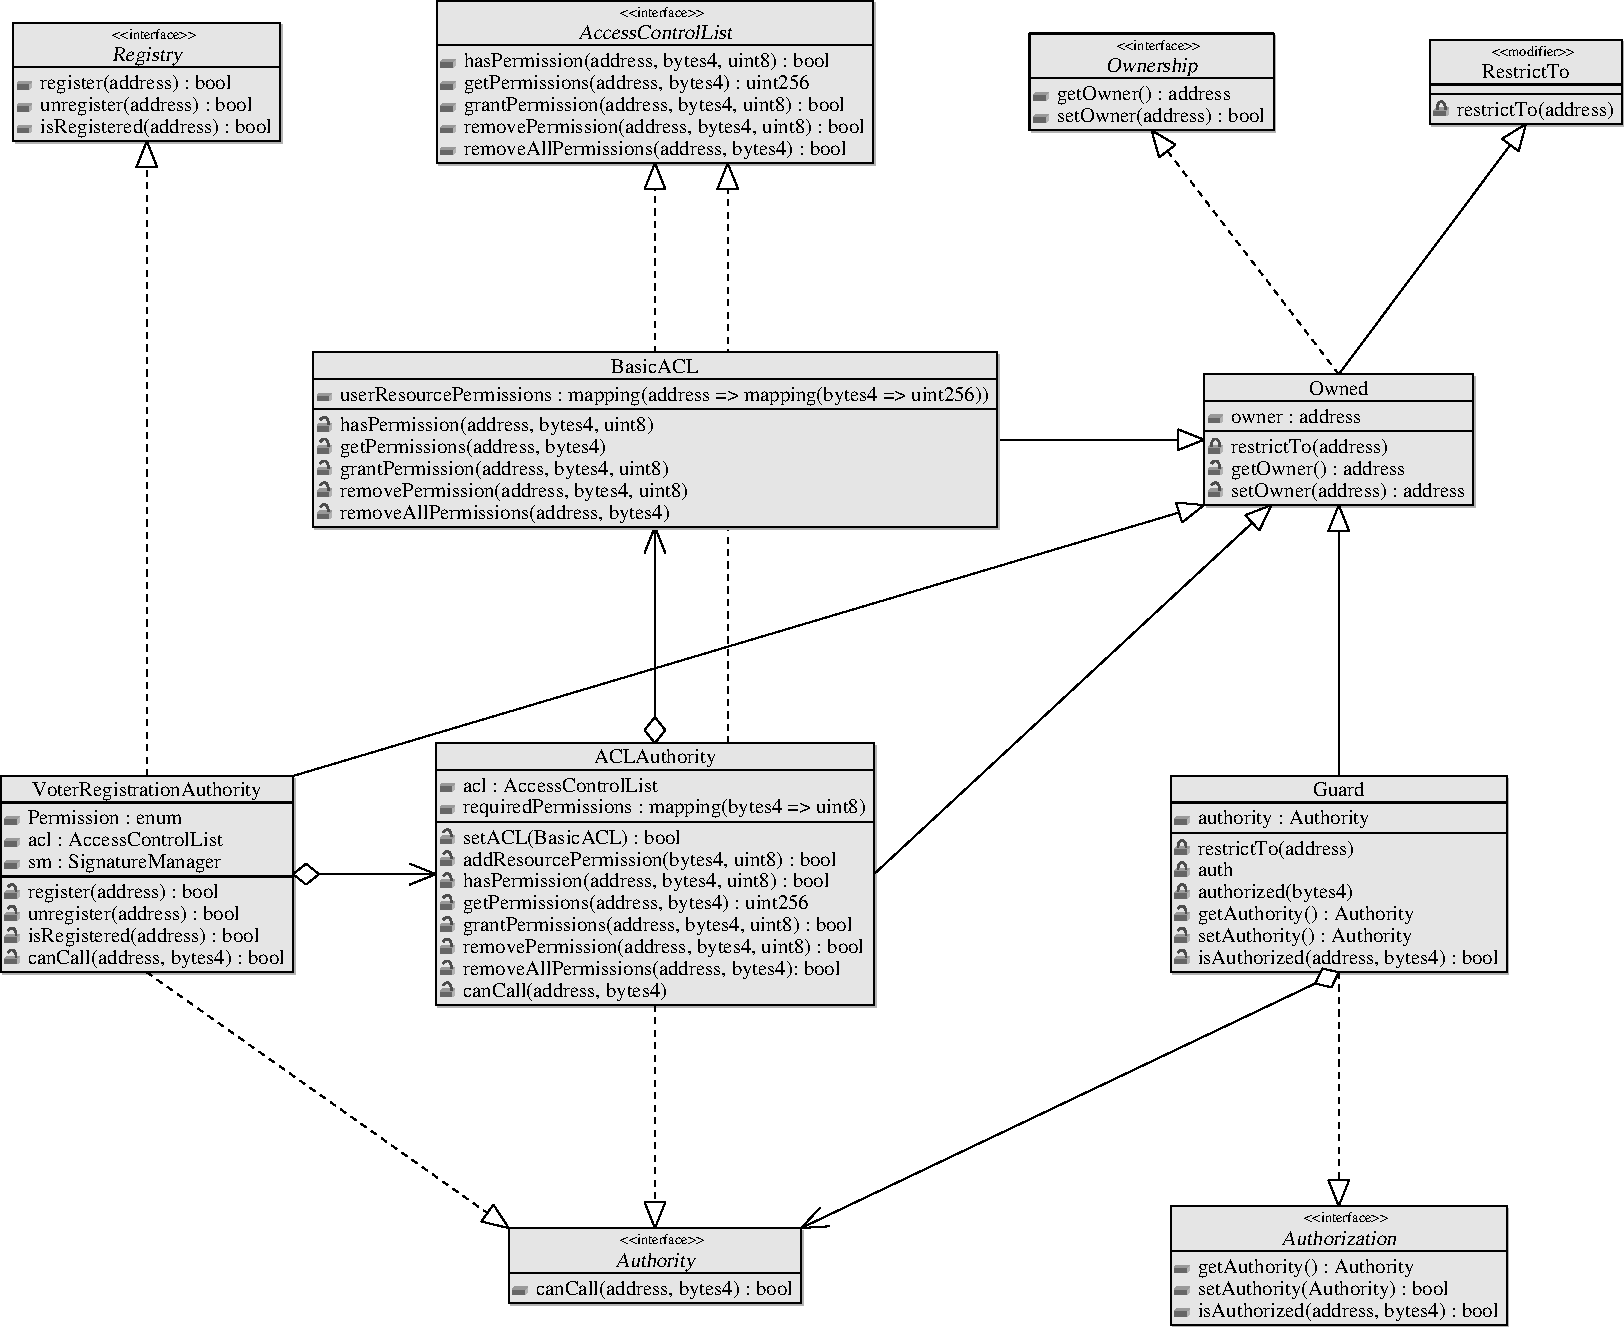
\includegraphics[width=\textwidth]{figures/authorization/figure}
  % \includestandalone[width=\textwidth]{\fig{authorization}}
\end{figure}

% Sub-sub-section: Managing Contract Ownership
\subsection{Primitive Contract Ownership}

Managing \solt{contract} ownership is one of the most basic forms of access
control in the Ethereum ecosystem. Here we introduce:

\begin{enumerate}
  \item \sol{interface Ownership}, which defines \solt{function}[s] to
    express \solt{contract} ownership,
  \item \sol{contract RestrictTo}, which defines a \solt{modifier} for
    restricting access to \solt{function} calls based on an \solt{address}, and
  \item \sol{contract Owned}, a convenience \solt{contract}, which provides an
    implementation of \sol{interface Ownership} and leverages
    \sol{contract RestrictTo}.
\end{enumerate}

\begin{figure}[H]
  \centering
  \caption{Contract ownership dependency graph modeling.}\label{fig:ownership}
  \figurepdf[]{ownership}
\end{figure}

\subsubsection{Contract RestrictTo}

The \solt{contract}, \sol{contract RestrictTo}, introduces a single
\solt{modifier}, \sol{modifier restrictTo}, which requires the caller of the
\solt{function}, \sol{msg.sender}, to have the same \solt{address} as the
argument, \sol{address _subject}, provided to the \solt{modifier} when called.

\begin{solidity}[contract RestrictTo]
contract RestrictTo {
  modifier restrictTo (address _subject) {
    require(msg.sender == _subject);
    _;
  }
}
\end{solidity}

\begin{code}
  \item \operations
  \begin{modifiers}
    \item \sol{modifier restrictTo (address _subject)}, restricts access to
      \solt{function} calls based on an \solt{address} provided.

      \begin{displayquote}
        Restriction to \solt{function}[s] is accomplished by comparing the
        \solt{address} of the \solt{function} \emph{caller}, \sol{msg.sender},
        against the configured \solt{address}, \sol{address _subject}. If the
        \solt{address} of the \solt{msg.sender} does not match the
        \solt{address} of the \solt{_subject} then the \solt{require} statement
        will force the immediately arrest of \solt{contract} evaluation,
        \solt{revert} the \emph{state} of the \solt{contract}, refund any
        remaining \solt{gas}, \solt{gasleft()}, to the \emph{caller}, and
        exit.\footnotemark{}

        \todo{Should notes be documented differently?}
      \end{displayquote}

      \footnotetext{
        Note that the \emph{caller}, \sol{msg.sender}, of the \solt{function}
        will not necessarily be an \emph{external account}, e.g., human user;
        the \emph{caller} of the \solt{contract} \solt{function} may itself also
        be a \solt{contract}, i.e., a \emph{contract account}, which is calling
        the \solt{contract} \solt{function} from its own \solt{contract}
        \solt{function}.
      }

      \begin{parameters}
      \item \sol{address _subject}, the \emph{subject} who is to be granted
        access to the \solt{function}.

        \begin{displayquote}
          The \solt{address} of the \emph{subject} may be \emph{any} Ethereum
          account, including \emph{contract accounts}.
        \end{displayquote}
      \end{parameters}
  \end{modifiers}
\end{code}


\paragraph{Interface Ownership}

The \solt{interface}, \sol{interface Ownership}, introduces two
\solt{function}[s] for managing contract ownership:

\begin{enumerate}
  \item \sol{function getOwner}, which is expected to return the \solt{address}
        of the owner of the \solt{contract}, and
  \item \sol{function setOwner}, which is expected to update the \solt{address}
        of the owner of the \solt{contract}.
\end{enumerate}

\begin{solidity}[interface Ownership]
interface Ownership {
  function getOwner () public view returns (address _owner);
  function setOwner (address _owner) public returns (bool _success);
}
\end{solidity}

\begin{interface}
\item \specification{}

  \begin{functions}
    \item \sol{function getOwner ()}, returns the \solt{address} of the owner of
      the \solt{contract}.

      \begin{returns}
        \item \sol{address _owner}, the \emph{subject} representing the owner of
          the \solt{contract}.
      \end{returns}

    \item \sol{function setOwner (address _owner)}, updates the \solt{address}
      representing the owner of the \solt{contract}.

      % which accepts an \solt{address},
      % \sol{address _owner}, and is expected to update the owner of the
      % \solt{contract} and \solt{return} a \solt{bool}, \sol{bool _success},
      % which resolves to \solt{true} if the operation was successful; otherwise
      % \solt{false}.


      \begin{parameters}
      \item \sol{address _owner}, the \emph{subject} which is to be granted
        ownership of the \solt{contract}.\footnotemark{}

        \footnotetext{\label{param:address-owner}
          The \solt{address} of the \emph{subject} may be \emph{any} Ethereum
          account, including \emph{contract accounts}.
        }
      \end{parameters}

      \begin{returns}
      \item \sol{bool _success}, resolves to \solt{true} if the operation was
        successful; otherwise \solt{false}.
      \end{returns}
  \end{functions}
\end{interface}


\subsubsection{Contract Owned}

A convenience \solt{contract}, \sol{contract Owned}, implements
\sol{interface Ownership} and extends \sol{contract RestrictTo}; in doing so,
\sol{contract Owned} provides a simple mechanism for expressing \solt{contract}
ownership, extending \sol{contract Owned}; e.g., \sol{contract MyContract is
Owned {}}.

% Upon creation, the \solt{constructor} of this \solt{contract} sets the
% \solt{owner} property of the \solt{contract} to the \solt{address} which
% created the contract, and restricts future calls to the \sol{function
% setOwner} to the owner of the \solt{contract} by using the \sol{modifier
% restrictTo(owner)}.

\begin{solidity}[contract Owned]
contract Owned is RestrictTo, Ownership {
  address public owner;

  constructor () {
    owner = msg.sender;
  }

  function getOwner () public view returns (address _owner) {
    return owner;
  }

  function setOwner (address _owner) public restrictTo(owner) returns (bool _success) {
    owner = _owner;
    return true;
  }
}
\end{solidity}

\begin{state}
  \item \attributes

  \begin{public}
    \item \sol{address owner}, maintains the \solt{address} of the current
      \solt{owner} of the \solt{contract}.
  \end{public}
\end{state}

\begin{code}
  \item \operations

  \begin{constructor}
    \item \sol{constructor ()}, upon creation and initialization of this
      \solt{contract} the \solt{constructor} sets the \sol{address owner}
      property of the \solt{contract} to the \solt{address} of the
      \solt{contract} creator, \sol{msg.sender}, i.e., the \emph{subject}
      submitting the \solt{CREATE} opcode.
  \end{constructor}

  \begin{functions}
    \item \sol{function getOwner ()}, returns the \solt{address} of the owner of
      the \solt{contract}.

      \begin{returns}
        \item \sol{address _owner}, the \emph{subject} representing the owner of
          the \solt{contract}.
      \end{returns}

    \item \sol{function setOwner (address _owner)}, updates the \solt{address}
      representing the owner of the \solt{contract}, effectively transferring
      ownership of the \solt{contract}.

      \begin{modifiers}
        \item \sol{modifier restrictTo (owner)}, restricts access to the
          \solt{function} such that \emph{only} the current \solt{owner} of the
          \solt{contract} can update/transfer ownership of the \solt{contract}.
      \end{modifiers}

      \begin{parameters}
        \item \sol{address _owner}, the \emph{subject} who is to be granted access
          to the \solt{function}.
      \end{parameters}

      \begin{returns}
        \item \sol{bool _success}, the \emph{subject} representing the owner of
          the \solt{contract}
      \end{returns}
  \end{functions}
\end{code}


% Sub-sub-section: Generalizing Contract Access Control
\subsection{Generalizing Contract Access Control}

In order to generalize \solt{contract} access control we introduce:

\begin{enumerate}
  \item \sol{interface Authority}, which defines \solt{function}[s] to determine
    whether some \emph{subject} is permitted to access some \emph{resource},
  \item \sol{contract Authorization}, which defines a \solt{modifier} for
    restricting access to \solt{function} calls based on an \solt{address}, and
  \item \sol{contract Guard}, a convenience \solt{contract}, which provides an
    implementation of \sol{interface Authorization} by aggregating
    implementations of \sol{interface Authority}.
\end{enumerate}

Together these components allow us to provide a generalized access control
model; isolating and deferring the responsibilities of
authorization.\footnotemark{}
\todo{Alternative names: Guard, Authority, Enforcer, Authorization}

\footnotetext{
  I think I would maybe prefer \sol{interface Authorization} to define
  \sol{isAuthorized} and for \sol{interface Authority} to define
  \sol{getAuthority} and \sol{setAuthority}.

  A better name in that case might be \sol{interface AuthorityManager}.
}

\begin{figure}[H]
  \centering
  \caption{Generalized contract access control.}% \label{fig:authorization}
  \figurepdf[]{guard}
  % 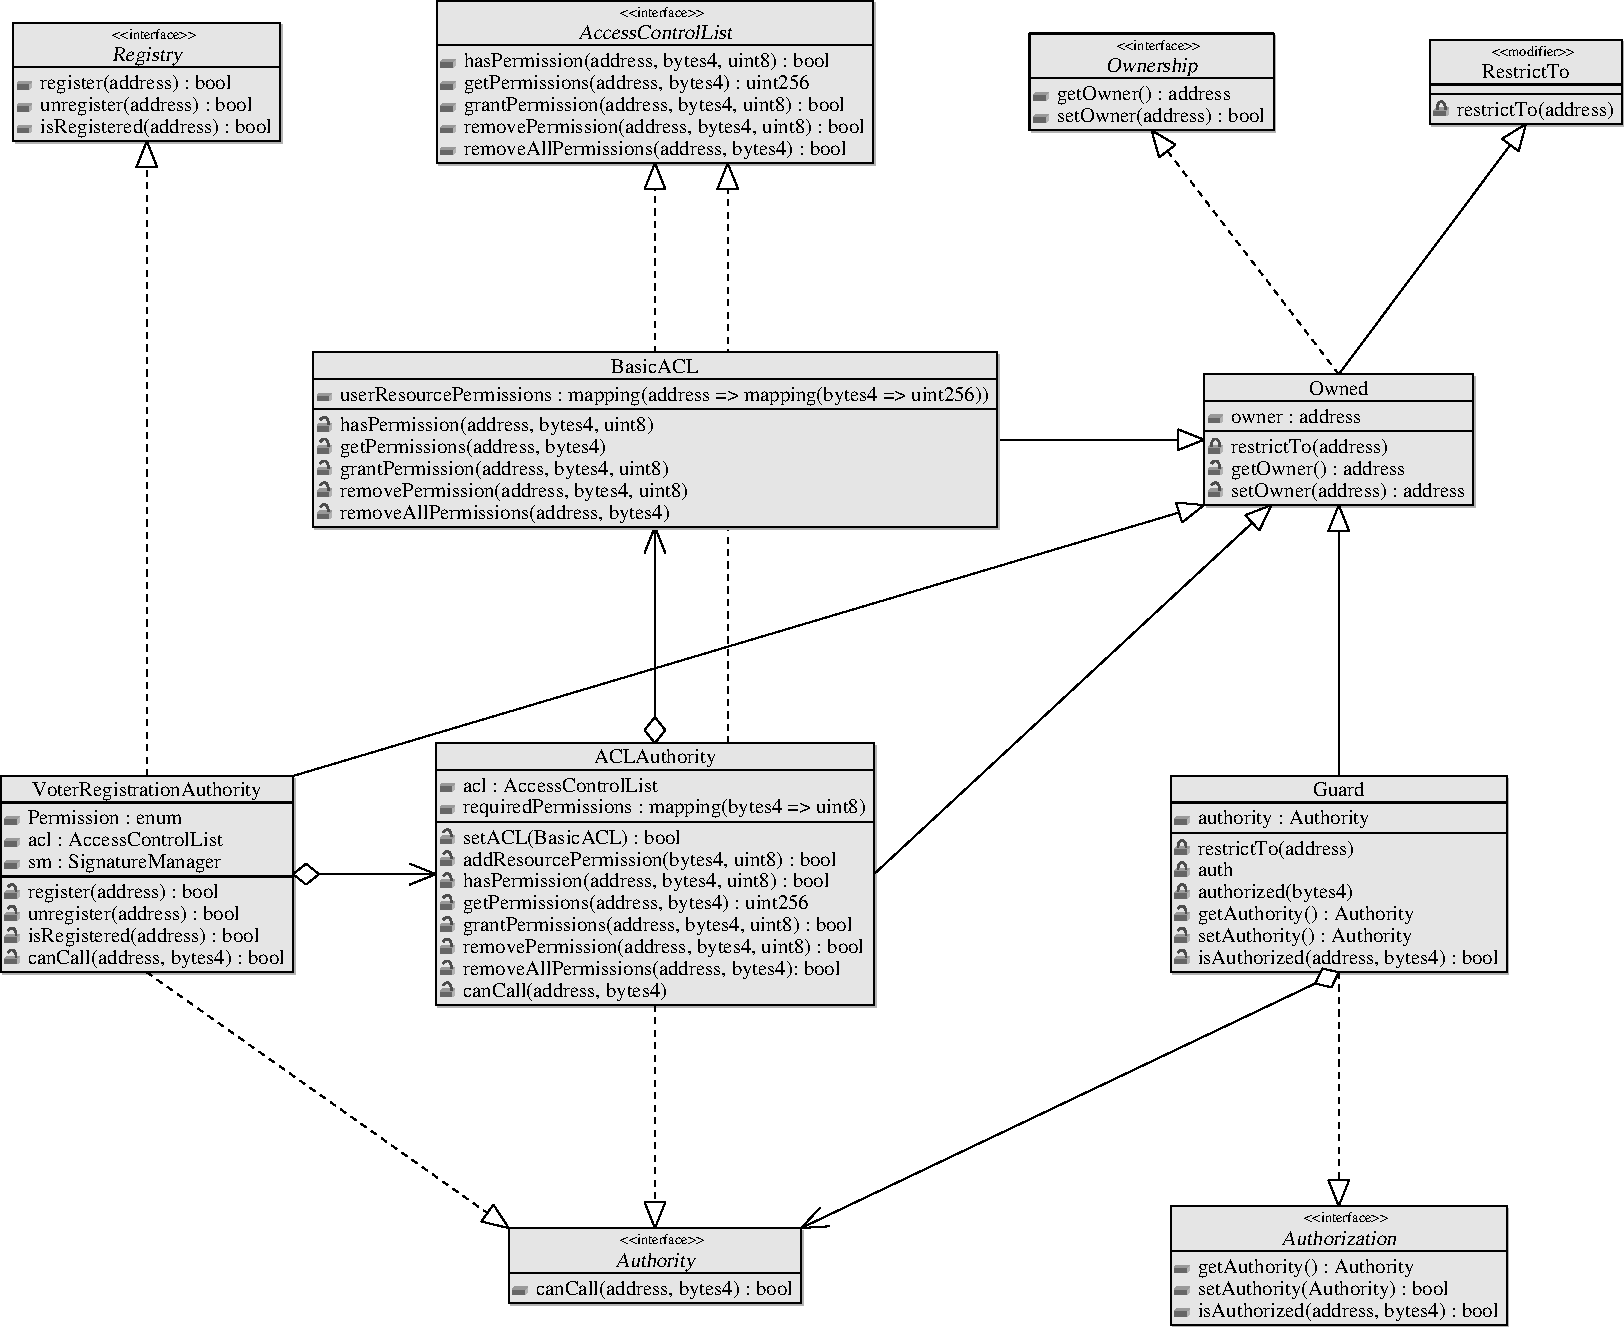
\includegraphics[width=\textwidth]{figures/authorization/figure}
  % \includestandalone[width=\textwidth]{\fig{authorization}}
\end{figure}

\subsubsection{Interface Authority}

The \solt{interface}, \sol{interface Authority}, introduces functionality for
managing whether some \emph{subject}, typically an Ethereum account represented
by \solt{address}, can access some \emph{resource}, typically an Ethereum
\solt{function} represented by \solt{function} signature, \solt{bytes4}. By
defining the \emph{resource} by it's \solt{function} signature and not by a
specific \solt{function} owned by a specific \solt{contract} we leave open the
possibility for managing \solt{contract} access control across
\solt{contract}[s], a functionality which will be necessary to build
pseudo-centralized registration authorities.

\begin{solidity}[interface Authority]
interface Authority {
  function canCall (address _subject, bytes4 _resource) public constant returns (bool _canCall);
}
\end{solidity}

\begin{interface}
  \item \specification{}

  \begin{functions}
    \item \sol{function canCall (address _subject, bytes4 _resource)}, evaluates
      whether some \emph{resource}, \solt{contract function}, can be used by
      some \emph{subject}, Ethereum account.

      \begin{parameters}
        \item \sol{address _subject}, the \emph{subject}, Ethereum account,
          whose permissions are being evaluated.\footnotemark{}

          \footnotetext{
            The \solt{address} of the \emph{subject} may be \emph{any} Ethereum
            account, including \emph{contract accounts}.
          }

        \item \sol{bytes4 _resource}, the \emph{resource}, \solt{contract
          function}, which the \emph{subject's} permissions are being evaluated
          against.
      \end{parameters}

      \begin{returns}
        \item \sol{bool _canCall}, resolves to \solt{true} if the
          \emph{subject}, \sol{address _subject}, is permitted to access the
          \emph{resource}, \sol{bytes4 _resource}, otherwise \solt{false}.
      \end{returns}
  \end{functions}
\end{interface}


\subsubsection{Interface Authorization}

The \solt{interface}, \sol{interface Authorization}, introduces functionality
for managing authorities, \sol{function getAuthority()} and \sol{function
setAuthority()}, and also functionality similar to that of an \solt{Authority},
\sol{function isAuthorized()}.\footnotemark{}

\footnotetext{
  If I don't update this to just be \sol{interface AuthorityManager} then I
  should \emph{really} update \sol{interface Authority} to supply \sol{function
  isAuthorized ()}, instead of \sol{function canCall()}, and update this
  \solt{interface} to implement/extend \sol{interface Authority}.
}

\begin{solidity}[interface Authorization]
interface Authorization {
  function getAuthority () public constant returns (address _authority);
  function setAuthority (address _authority) public returns (bool _success);
  function isAuthorized (address _subject, bytes4 _resource) public returns (bool _isAuthorized);
}
\end{solidity}

\begin{interface}
\item \specification{}

  \begin{functions}
    \item \sol{function getAuthority ()}, returns the \solt{address} of a
      \solt{contract} which implements the \solt{interface Authority}.

      \begin{returns}
        \item \sol{address _authority}, the \solt{address} of a \solt{contract}
          which implments the \solt{interface Authority}.
      \end{returns}

    \item \sol{function setAuthority (address _authority)}, updates the state of
      the \solt{contract} to to reflect the new \solt{contract} which provides
      an implementation of the \solt{Authority interface}.

      \todo{Make sure the Guard checks that the contract actually implements the
      interface!!!}

      \begin{parameters}
        \item \sol{address _authority}, the \solt{address} of a \solt{contract}
          which implements the \solt{interface Authority}.
      \end{parameters}

      \begin{returns}
        \item \sol{bool _success}, resolves to \solt{true} if the operation was
          successful; otherwise \solt{false}.
      \end{returns}

    \item \sol{function isAuthorized (address _subject, bytes4 _resource)},
      evaluates whether some \emph{subject}, Ethereum account, is authorized to
      access some \emph{resource}, \solt{contract function}.

      \begin{parameters}
        \item \sol{address _subject}, the \emph{subject}, Ethereum account,
          whose permissions are being evaluated.\footnotemark{}

          \footnotetext{
            The \solt{address} of the \emph{subject} may be \emph{any} Ethereum
            account, including \emph{contract accounts}.
          }

        \item \sol{bytes4 _resource}, the \emph{resource}, \solt{contract
          function}, which the \emph{subject's} permissions are being evaluated
          against.
      \end{parameters}

      \begin{returns}
        \item \sol{bool _isAuthorized}, resolves to \solt{true} if the
          \emph{subject}, \sol{address _subject}, is permitted to access the
          \emph{resource}, \sol{bytes4 _resource}, otherwise \solt{false}.
      \end{returns}
  \end{functions}
\end{interface}


\subsubsection{Contract Guarded}

The \solt{contract}, \sol{contract Guarded}, is a \solt{contract} which offers a
convenient mechanism for easily integrating generalized \solt{contract} access
control functionality; e.g., \sol{contract MyContract is Guarded {}}.
\solt{contract Guarded}, by virtue of implementing the \solt{Authorization
interface}, supports deferring access control responsibilities to an external
\solt{contract} which implements the \solt{Authority interface} while leaving
open the possibility for a \solt{contract} to provide its own access control
implementation by itself implementing the \solt{Authority interface}.

\todo{If I'm changing this from Guard to Guarded then I need to update all of
the references to Guard.}

\begin{solidity}[contract Guarded]
contract Guarded is Owned, Authorization {
  Authority public authority;

  function getAuthority () public constant returns (address _authority) {
    return address(authority);
  }

  function setAuthority (address _authority) public auth returns (bool _success) {
    authority = Authority(_authority);
    return true;
  }

  function isAuthorized (address _subject, bytes4 _resource) public returns (bool _isAuthorized) {
    if (_subject == address(this)) return true;
    if (authority == Authority(0)) return false;
    if (_subject == owner) return true;
    return authority.canCall(_subject, _resource);
  }

  modifier auth {
    assert(isAuthorized(msg.sender, msg.sig));
    _;
  }

  modifier authorized (bytes4 _resource) {
    assert(isAuthorized(msg.sender, _resource));
    _;
  }
}
\end{solidity}

\begin{code}
  \item \operations
  \begin{modifiers}
    \item \sol{modifier auth ()}, restricts access to \solt{function} calls
      based on an \solt{address} provided.

      \begin{displayquote}
        Restriction to \solt{function}[s] is accomplished by comparing the
        \solt{address} of the \solt{function} \emph{caller}, \sol{msg.sender},
        against the configured \solt{address}, \sol{address _subject}. If the
        \solt{address} of the \solt{msg.sender} does not match the
        \solt{address} of the \solt{_subject} then the \solt{require} statement
        will force the immediately arrest of \solt{contract} evaluation,
        \solt{revert} the \emph{state} of the \solt{contract}, refund any
        remaining \solt{gas}, \solt{gasleft()}, to the \emph{caller}, and
        exit.\footnotemark{}

        \todo{Should notes be documented differently?}
      \end{displayquote}

      \footnotetext{
        Note that the \emph{caller}, \sol{msg.sender}, of the \solt{function}
        will not necessarily be an \emph{external account}, e.g., human user;
        the \emph{caller} of the \solt{contract} \solt{function} may itself also
        be a \solt{contract}, i.e., a \emph{contract account}, which is calling
        the \solt{contract} \solt{function} from its own \solt{contract}
        \solt{function}.
      }

      \begin{parameters}
      \item \sol{address _subject}, the \emph{subject} who is to be granted
        access to the \solt{function}.

        \begin{displayquote}
          The \solt{address} of the \emph{subject} may be \emph{any} Ethereum
          account, including \emph{contract accounts}.
        \end{displayquote}
      \end{parameters}

    \item \sol{modifier authorized (address _resource)}, restricts access to
      \solt{function} calls based on an \solt{address} provided.

      \begin{displayquote}
        Restriction to \solt{function}[s] is accomplished by comparing the
        \solt{address} of the \solt{function} \emph{caller}, \sol{msg.sender},
        against the configured \solt{address}, \sol{address _subject}. If the
        \solt{address} of the \solt{msg.sender} does not match the
        \solt{address} of the \solt{_subject} then the \solt{require} statement
        will force the immediately arrest of \solt{contract} evaluation,
        \solt{revert} the \emph{state} of the \solt{contract}, refund any
        remaining \solt{gas}, \solt{gasleft()}, to the \emph{caller}, and
        exit.\footnotemark{}

        \todo{Should notes be documented differently?}
      \end{displayquote}

      \footnotetext{
        Note that the \emph{caller}, \sol{msg.sender}, of the \solt{function}
        will not necessarily be an \emph{external account}, e.g., human user;
        the \emph{caller} of the \solt{contract} \solt{function} may itself also
        be a \solt{contract}, i.e., a \emph{contract account}, which is calling
        the \solt{contract} \solt{function} from its own \solt{contract}
        \solt{function}.
      }

      \begin{parameters}
      \item \sol{address _subject}, the \emph{subject} who is to be granted
        access to the \solt{function}.

        \begin{displayquote}
          The \solt{address} of the \emph{subject} may be \emph{any} Ethereum
          account, including \emph{contract accounts}.
        \end{displayquote}
      \end{parameters}
  \end{modifiers}
\end{code}


% Sub-sub-section: Access Control Lists
\subsection{Access Control Lists}

We introduce access control lists to provide a generalized form of access
control through a well-understood and common interface:

\begin{enumerate}
  \item \sol{interface AccessControlList}, which defines the basic actions
    required for an access control list implementation;

  \item \sol{contract BasicACL}, which provides a basic implementation of
    \sol{interface AccessControlList}; and

  \item \sol{contract ACLAuthority}, which aggregates an
    \solt{interface AccessControlList} implementation, \sol{contract BasicACL}
    in this case, to back an \sol{interface Authority} implementation.
\end{enumerate}

\begin{figure}[H]
  \centering
  \caption{Generalized contract access control by way of access control lists.}\label{fig:acl}
  \figurepdf[]{access-control-lists}
  % 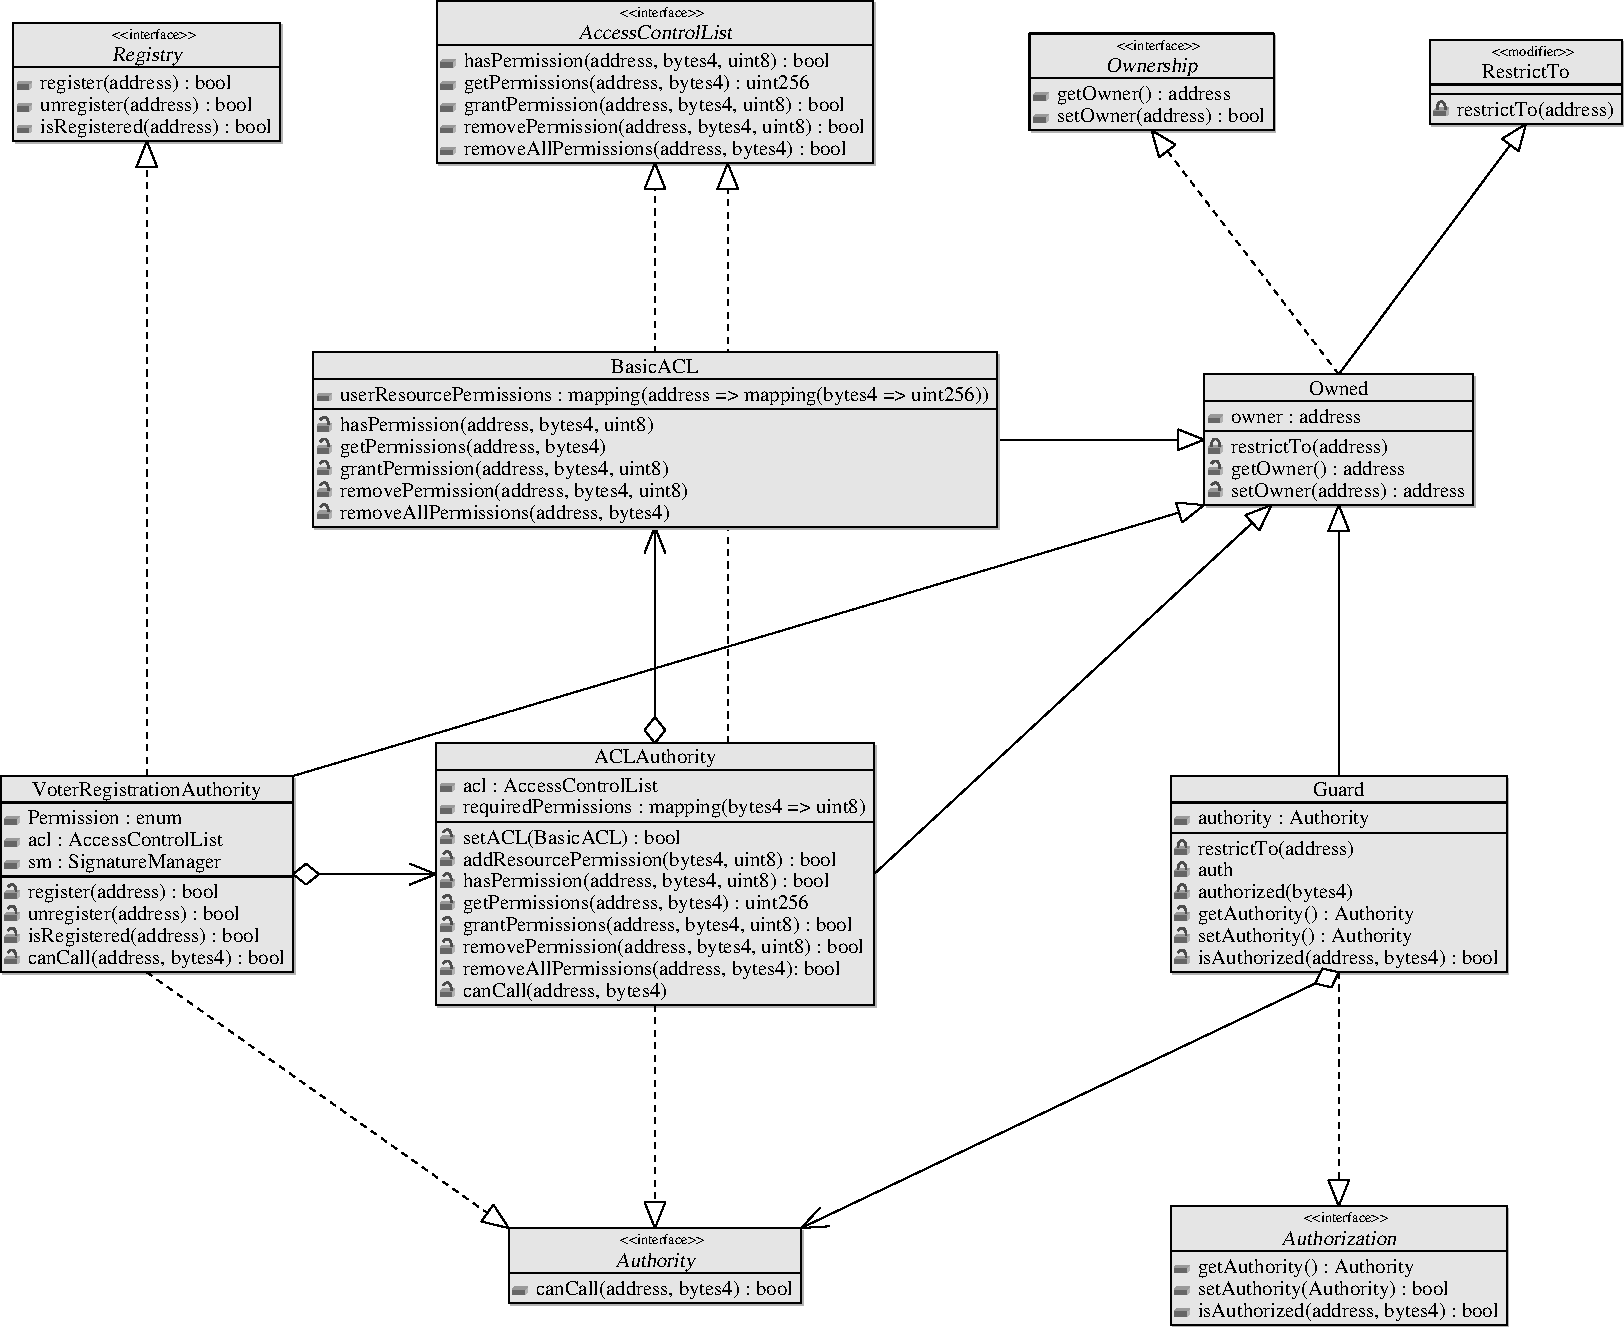
\includegraphics[width=\textwidth]{figures/authorization/figure}
  % \includestandalone[width=\textwidth]{\fig{authorization}}
\end{figure}

\subsubsection{Interface AccessControlList}

The \solt{interface}, \sol{interface AccessControlList}, introduces five
\solt{function} definitions to achieve basic access control list functionality:

\begin{enumerate}
  \item \sol{function hasPermission}, which validates that a \emph{subject} has
    the \emph{permission} required access some \emph{resource}.

  \item \sol{function getPermissions}, which returns the \emph{permissions} some
    \emph{subject} has for a given \emph{resource}.

  \item \sol{function setPermissions}, which updates the \emph{permissions} some
    \emph{subject} has for a given \emph{resource}.

  \item \sol{function grantPermission}, which grants a single \emph{permission}
    for some \emph{subject} with respect to some \emph{resource}.

  \item \sol{function revokePermission}, which revokes a single
    \emph{permission} for some \emph{subject} with respect to some
    \emph{resource}.
\end{enumerate}

\begin{solidity}[interface AccessControlList]
interface AccessControlList {
  function hasPermission (address _subject, bytes4 _resource, uint8 _permission)
    public view returns (bool _hasPermission);

  function getPermissions (address _subject, bytes4 _resource)
    public view returns (uint256 _permissions);

  function setPermissions (address _subject, bytes4 _resource, uint256 _permissions)
    public returns (bool _success);

  function grantPermission (address _subject, bytes4 _resource, uint8 _permission)
    public returns (bool _success);

  function revokePermission (address _subject, bytes4 _resource, uint8 _permission)
    public returns (bool _success);
}
\end{solidity}

\begin{interface}
  \item \specification{}
  \begin{functions}
    \item \sol{function hasPermission (address _subject, bytes4 _resource, uint8 _permission)},
      evaluates whether some \emph{subject} has the requisite \emph{permission}
      to access some \emph{resource}.

      \begin{parameters}
        \item \sol{address _subject}, the \solt{address} of an account
          representing the \emph{subject}, i.e., the \emph{user}, to evaluate
          permissions against.
        \item \sol{bytes4 _resource}, the \emph{resource}, signature hash of a
          Solidity \solt{function}, to validate \emph{permissions} against.
        \item \sol{uint8 _permission}, a \emph{permission} level, or
          \emph{action}, which is being validated.
      \end{parameters}

      \begin{returns}
        \item \sol{bool _hasPermission}, returns the \solt{true} if the
          \emph{subject} has the requisite \emph{permission} to access the
          \emph{resource}, otherwise \solt{false}.
      \end{returns}

    \item \sol{function getPermissions (address _subject, bytes4 _resource)},
      retrieves the \emph{permissions}, for a \emph{<subject, resource>} pair.

      \begin{parameters}
        \item \sol{address _subject}, the account \solt{address} of the
          \emph{subject} whose \emph{permissions} are to be retrieved.

        \item \sol{bytes4 _resource}, the \emph{resource}, \solt{function}
          signature, which the \emph{permissions} should be retrieved for.
      \end{parameters}

      \begin{returns}
      \item \sol{uint256 _permissions}, the \solt{uint256} representation of the
        \emph{subject's} \emph{permissions} for a given \emph{resource}.
      \end{returns}

    \item \sol{function setPermissions (address _subject, bytes4 _resource, uint256 _permissions)},
      updates a \emph{subject's} \emph{permissions} for some \emph{resource}.

      \begin{parameters}
        \item \sol{address _subject}, the account \solt{address} of the
          \emph{subject} whose \emph{permissions} are to be modified.

        \item \sol{bytes4 _resource}, the \emph{resource}, \solt{function}
          signature, which the \emph{permissions} are to be modified for.

        \item \sol{uint256 _permissions}, the \solt{uint256} representation of
          the \emph{subject's} new \emph{permissions} for the \emph{resource}.
      \end{parameters}

      \begin{returns}
      \item \sol{bool _success}, resolves to \solt{true} if the operation was
        successful, otherwise \solt{false}.
      \end{returns}

    \item \sol{function grantPermission (address _subject, bytes4 _resource, uint8 _permission)},
      grants a \emph{subject} some \emph{permission} for a given \emph{resource}.

      \begin{parameters}
        \item \sol{address _subject}, the account \solt{address} of the
          \emph{subject} whose \emph{permissions} are to be modified.

        \item \sol{bytes4 _resource}, the \emph{resource}, \solt{function}
          signature, which the \emph{permissions} are to be modified for.

        \item \sol{uint8 _permission}, a \solt{uint8} value representing the
          \emph{permission-bit} to enable for the \emph{<subject, resource>}
          pair.
      \end{parameters}

      \begin{returns}
      \item \sol{bool _success}, resolves to \solt{true} if the operation was
        successful, otherwise \solt{false}.
      \end{returns}

    \item \sol{function revokePermission (address _subject, bytes4 _resource, uint8 _permission)},
      revokes a \emph{subject's} \emph{permission} for a given \emph{resource}.

      \begin{parameters}
        \item \sol{address _subject}, the account \solt{address} of the
          \emph{subject} whose \emph{permissions} are to be modified.

        \item \sol{bytes4 _resource}, the \emph{resource}, \solt{function}
          signature, which the \emph{permissions} are to be modified for.

        \item \sol{uint8 _permission}, a \solt{uint8} value representing the
          \emph{permission-bit} to revoke for the \emph{<subject, resource>}
          pair.
      \end{parameters}

      \begin{returns}
      \item \sol{bool _success}, resolves to \solt{true} if the operation was
        successful, otherwise \solt{false}.
      \end{returns}
  \end{functions}
\end{interface}

% \paragraph{function hasPermission}
%
% \subparagraph{Parameters}
% \begin{enumerate}
%   \item \sol{address _subject}, which represents some \emph{subject}, or
%         \emph{user}, accessing some \emph{resource}.
%   \item \sol{bytes4 _resource}, a \emph{resource}, or Solidity
%         \solt{function}, to validate \emph{permissions} against.
%   \item \sol{uint8 _permission}, a \emph{permission} level, or \emph{action},
%         which is being validated.
% \end{enumerate}
%
% \subparagraph{Returns}
% \sol{function hasPermission} is expected to \solt{return} a \solt{bool},
% \sol{bool _hasPermission}, which resolves to \solt{true} if the
% \emph{subject} has permission to access the \emph{resource}, Solidity
% \solt{function} associated with \sol{bytes4 _resource}, at the
% \emph{permission} level specified by \sol{uint8 _permission}.
%
% \paragraph{function getPermissions}
% \subparagraph{Parameters}
% \subparagraph{Returns}
%
% \paragraph{function setPermissions}
% \subparagraph{Parameters}
% \subparagraph{Returns}
%
% \paragraph{function grantPermission}
% \subparagraph{Parameters}
% \subparagraph{Returns}
%
% \paragraph{function removePermission}
% \subparagraph{Parameters}
% \subparagraph{Returns}
%


\subsubsection{Contract BasicACL}

The \solt{contract}, \sol{contract BasicACL}, implements the ACL
\solt{interface}, \sol{interface AccessControlList}, to provide a primitive
ACL implementation. The \solt{contract} implementation is backed by a mapping of
references, from \emph{subject} to \emph{resource} to \emph{permissions} --- as
described in Chapter~\ref{chap:methods}, \emph{\nameref{chap:methods}} --- i.e.,
a nested sparse vector mapping.

\begin{solidity}[contract BasicACL]
contract BasicACL is Owned, AccessControlList {
  mapping (address => mapping (bytes4 => uint256)) subjectResourcePermissions;

  function hasPermission (address _subject, bytes4 _resource, uint8 _permission) public constant restrictTo(owner) returns (bool _hasPermission) {
    uint256 result = subjectResourcePermissions[_subject][_resource] & (uint256(1) << _permission);
    return (result > 0);
  }

  function getPermissions (address _subject, bytes4 _resource) public constant restrictTo(owner) returns (uint256 _permissions) {
    return subjectResourcePermissions[_subject][_resource];
  }

  function grantPermission (address _subject, bytes4 _resource, uint8 _permission) public restrictTo(owner) returns (bool _success) {
    subjectResourcePermissions[_subject][_resource] |= uint256(1) << _permission;
    return true;
  }

  function revokePermission (address _subject, bytes4 _resource, uint8 _permission) public restrictTo(owner) returns (bool _success) {
    subjectResourcePermissions[_subject][_resource] &= ~(uint256(1) << _permission);
    return true;
  }

  function setPermissions (address _subject, bytes4 _resource, _permissions) public restrictTo(owner) returns (bool _success) {
    subjectResourcePermissions[_subject][_resource] = _permissions;
    return true;
  }
}
\end{solidity}

\begin{state}
  \item \attributes

  \begin{public}
    \item \sol{mapping (address => mapping (bytes4 => uint256)) subjectResourcePermissions}
      a nesting mapping used to record the \emph{permissions} which
      \emph{subjects} have to access various \emph{resources}.

      \begin{displayquote}
        Here \emph{subjects} are represented and identified by their account
        \solt{address}; \emph{resources} are assumed to be \solt{function}
        signatures, \solt{bytes4}; and \emph{permissions} are bit vectors,
        backed by \solt{uint256} values, where bit masks are leveraged to
        retrieve individual \emph{permission} values.
      \end{displayquote}
  \end{public}
\end{state}

\begin{code}
  \item \operations

  \begin{functions}
    \item \sol{function hasPermission (address _subject, bytes4 _resource, uint8 _permission)},
      evaluates whether some \emph{subject} has the requisite \emph{permission}
      to access some \emph{resource}.

      \begin{displayquote}
        \emph{Permission} evaluation occurs by:
        \begin{enumerate}
          \item retrieving the \emph{permissions} bit vector from the
            \solt{mapping} \sol{subjectResourcePermissions}, where the
            \emph{subject}, \sol{address _subject}, and \emph{resource},
            \sol{bytes4 _resource}, are used as keys;

          \item creating a \emph{permission} bit mask by left-shifting 1
            \sol{_permission} times, \sol{1 << _permission};

          \item evaluating \sol{permissions |$\land$| bit_mask}; and finally,

          \item returning \solt{true} if the value resulting from the evaluation
            is greater than 0, i.e., the \emph{subject} has \emph{permission} to
            access to the \emph{resource}.
        \end{enumerate}
      \end{displayquote}

      \begin{parameters}
        \item \sol{address _subject}, the \solt{address} of an account
          representing the \emph{subject}, i.e., the \emph{user}, to evaluate
          permissions against.
        \item \sol{bytes4 _resource}, the \emph{resource}, signature hash of a
          Solidity \solt{function}, to validate \emph{permissions} against.
        \item \sol{uint8 _permission}, a \emph{permission} level, or
          \emph{action}, which is being validated.
      \end{parameters}

      \begin{returns}
        \item \sol{bool _hasPermission}, returns the \solt{true} if the
          \emph{subject} has the requisite \emph{permission} to access the
          \emph{resource}, otherwise \solt{false}.
      \end{returns}

    \item \sol{function getPermissions (address _subject, bytes4 _resource)},
      retrieves the \emph{permissions}, for a \emph{<subject, resource>} pair.

      \begin{parameters}
        \item \sol{address _subject}, the account \solt{address} of the
          \emph{subject} whose \emph{permissions} are to be retrieved.

        \item \sol{bytes4 _resource}, the \emph{resource}, \solt{function}
          signature, which the \emph{permissions} should be retrieved for.
      \end{parameters}

      \begin{returns}
      \item \sol{uint256 _permissions}, the \solt{uint256} representation of the
        \emph{subject's} \emph{permissions} for a given \emph{resource}.
      \end{returns}

    \item \sol{function setPermissions (address _subject, bytes4 _resource, uint256 _permissions)},
      updates a \emph{subject's} \emph{permissions} for some \emph{resource}.

      \begin{modifiers}
        \item \sol{modifier restrictTo (owner)}, restricts access to the
          \solt{function} such that \emph{only} the current \solt{owner} of the
          \solt{contract} can call it.
      \end{modifiers}

      \begin{parameters}
        \item \sol{address _subject}, the account \solt{address} of the
          \emph{subject} whose \emph{permissions} are to be modified.

        \item \sol{bytes4 _resource}, the \emph{resource}, \solt{function}
          signature, which the \emph{permissions} are to be modified for.

        \item \sol{uint256 _permissions}, the \solt{uint256} representation of
          the \emph{subject's} new \emph{permissions} for the \emph{resource}.
      \end{parameters}

      \begin{returns}
        \item \sol{bool _success}, resolves to \solt{true} if the operation was
          successful, otherwise \solt{false}.
      \end{returns}

    \item \sol{function grantPermission (address _subject, bytes4 _resource, uint8 _permission)},
      grants a \emph{subject} \emph{permission} for a given \emph{resource}.

      \begin{displayquote}
        \emph{Permission} grant occurs by:
        \begin{enumerate}
          \item retrieving the \emph{permissions} bit vector from the
            \solt{mapping} \sol{subjectResourcePermissions}, where the
            \emph{subject}, \sol{address _subject}, and \emph{resource},
            \sol{bytes4 _resource}, are used as keys;

          \item creating a \emph{permission} bit mask by left-shifting 1
            \sol{_permission} times, \sol{1 << _permission};

          \item evaluating \sol{permissions |$\lor$| bit_mask} to produce a new
            \emph{permissions} bit vector; and finally,

          \item updating the state of the \solt{contract} by storing the
            resulting \emph{permissions} bit vector back into the
            \sol{subjectResourcePermissions} \solt{mapping}.
        \end{enumerate}
      \end{displayquote}

      \begin{modifiers}
        \item \sol{modifier restrictTo (owner)}, restricts access to the
          \solt{function} such that \emph{only} the current \solt{owner} of the
          \solt{contract} can call it.
      \end{modifiers}

      \begin{parameters}
        \item \sol{address _subject}, the account \solt{address} of the
          \emph{subject} whose \emph{permissions} are to be modified.

        \item \sol{bytes4 _resource}, the \emph{resource}, \solt{function}
          signature, which the \emph{permissions} are to be modified for.

        \item \sol{uint8 _permission}, a \solt{uint8} value representing the
          \emph{permission-bit} to enable for the \emph{<subject, resource>}
          pair.
      \end{parameters}

      \begin{returns}
      \item \sol{bool _success}, resolves to \solt{true} if the operation was
        successful, otherwise \solt{false}.
      \end{returns}

    \item \sol{function revokePermission (address _subject, bytes4 _resource, uint8 _permission)},
      revokes a \emph{subject's} \emph{permission} for a given \emph{resource}.

      \begin{displayquote}
        \emph{Permission} revocation occurs by:
        \begin{enumerate}
          \item retrieving the \emph{permissions} bit vector from the
            \solt{mapping} \sol{subjectResourcePermissions}, where the
            \emph{subject}, \sol{address _subject}, and \emph{resource},
            \sol{bytes4 _resource}, are used as keys;

          \item creating a \emph{permission} bit mask by left-shifting 1
            \sol{_permission} times, \sol{1 << _permission};

          \item flipping all of the bits of the \emph{permission} bit mask,
            \sol{~bit_mask};

          \item evaluating \sol{permissions |$\land$| bit_mask} to produce a new
            \emph{permissions} bit vector; and finally,

          \item updating the state of the \solt{contract} by storing the
            resulting \emph{permissions} bit vector back into the
            \sol{subjectResourcePermissions} \solt{mapping}.
        \end{enumerate}
      \end{displayquote}

      \begin{modifiers}
        \item \sol{modifier restrictTo (owner)}, restricts access to the
          \solt{function} such that \emph{only} the current \solt{owner} of the
          \solt{contract} can call it.
      \end{modifiers}

      \begin{parameters}
        \item \sol{address _subject}, the account \solt{address} of the
          \emph{subject} whose \emph{permissions} are to be modified.

        \item \sol{bytes4 _resource}, the \emph{resource}, \solt{function}
          signature, which the \emph{permissions} are to be modified for.

        \item \sol{uint8 _permission}, a \solt{uint8} value representing the
          \emph{permission-bit} to revoke for the \emph{<subject, resource>}
          pair.
      \end{parameters}

      \begin{returns}
      \item \sol{bool _success}, resolves to \solt{true} if the operation was
        successful, otherwise \solt{false}.
      \end{returns}
  \end{functions}
\end{code}


\subsubsection{Contract ACLAuthority}

The \solt{contract}, \sol{contract ACLAuthority}, merges the ACL functionality
introduced by \sol{interface AccessControlList} with the generalized access
control functionality introduced by \sol{interface Authority}.

\begin{solidity}[contract ACLAuthority]
contract ACLAuthority is Owned, Authority, AccessControlList {
  AccessControlList acl;
  mapping (bytes4 => uint8) requiredResourcePermission;

  constructor (bool _createACL) {
    if (_createACL) acl = new BasicACL();
  }

  function hasPermission (address _subject, bytes4 _resource, uint8 _permission) public constant returns (bool _hasPermission) {
    return acl.hasPermission(_subject, _resource, _permission);
  }

  function getPermissions (address _subject, bytes4 _resource) public constant returns (uint256 _permissions) {
    return acl.getPermissions(_subject, _resource);
  }

  function grantPermission (address _subject, bytes4 _resource, uint8 _permission) public restrictTo(owner) returns (bool _success) {
    return acl.grantPermission(_subject, _resource, _permission);
  }

  function revokePermission (address _subject, bytes4 _resource, uint8 _permission) public restrictTo(owner) returns (bool _success) {
    return acl.removePermission(_subject, _resource, _permission);
  }

  function setPermissions (address _subject, bytes4 _resource, uint256 _permissions) public restrictTo(owner) returns (bool _success) {
    return acl.setPermissions(_subject, _resource, _permissions);
  }

  function setACL(AccessControlList _acl) public restrictTo(owner) returns (bool _success) {
    assert(_acl.owner() == address(this));
    acl = _acl;
    return true;
  }

  function setRequiredResourcePermission (bytes4 _resource, uint8 _permission) public restrictTo(owner) returns (bool _success) {
    requiredResourcePermission[_resource] = _permission;
    return true;
  }

  function canCall (address _subject, bytes4 _resource) public constant returns (bool _canCall) {
    return hasPermission(_subject, _resource, requiredResourcePermission[_sig]);
  }
}
\end{solidity}

\begin{state}
  \item \attributes

  \begin{public}
    \item \sol{AccessControlList acl} maintains the \solt{address} of an ACL
      implementation, a \solt{contract} which implements \sol{interface
      AccessControlList}.

    \item \sol{mapping (bytes4 => uint8) requiredResourcePermissions} maintains a
      mapping of \solt{function}[s], \sol{bytes4}, to required
      \emph{permission}, \sol{uint8}.
  \end{public}
\end{state}

\begin{code}
  \item \operations

  \begin{constructor}
    \item \sol{constructor (bool _createACL)}, upon creation and initialization
      of this \solt{contract} the \solt{constructor} can deploy a
      \solt{contract}, \sol{contract BasicACL}, if the \solt{bool}, \sol{bool
      _createACL}, is set to \solt{true}.

      \begin{parameters}
      \item \sol{bool _createACL}, set to \solt{true} to deploy an ACL
        implementation, \sol{contract BasicACL}, in addition to this
        \solt{contract}; otherwise \solt{false}.
      \end{parameters}
  \end{constructor}

  \begin{functions}
    \item \sol{function setAcl (AccessControlList _acl)}, updates the
      \solt{contract} reference which is responsible for managing ACL requests.

      \begin{modifiers}
        \item \sol{modifier restrictTo (owner)}, restricts access to the
          \solt{function} such that \emph{only} the current \solt{owner} of the
          \sol{contract} can call it.
      \end{modifiers}

      \begin{parameters}
        \item \sol{AccessControlList _acl}, the ACL implementation which access
          control responsibilities are to be delegated to.
      \end{parameters}

      \begin{returns}
        \item \sol{bool _success}, resolves to \solt{true} if the operation was
          successful, otherwise \solt{false}.
      \end{returns}


    \item \sol{function setRequiredResourcePermission (bytes4 _resource, uint8 _permission)},
      updates the mapping representing the \emph{permission} required to access
      some \emph{resource}, \solt{function} signature.

      \begin{modifiers}
        \item \sol{modifier restrictTo (owner)}, restricts access to the
          \solt{function} such that \emph{only} the current \solt{owner} of the
          \sol{contract} can call it.
      \end{modifiers}

      \begin{parameters}
        \item \sol{bytes4 _resource}, the \emph{resource}, \solt{function}
          signature, which the \emph{permission} is to be modified for.

        \item \sol{uint8 _permission}, a \solt{uint8} value representing the
          \emph{permission-bit} required for the \emph{resource}.
      \end{parameters}

      \begin{returns}
        \item \sol{bool _success}, resolves to \solt{true} if the operation was
          successful, otherwise \solt{false}.
      \end{returns}


    \item \sol{function canCall (address _subject, bytes4 _resource)}, evaluates
      whether a \emph{subject} can access to some \emph{resource} by validating
      with the ACL implementation that the \emph{subject} has the required
      \emph{resource} \emph{permission}.

      \begin{parameters}
        \item \sol{address _subject}, the \emph{subject}, Ethereum account,
          whose \emph{permissions} are being evaluated.

        \item \sol{bytes4 _resource}, the \emph{resource}, \solt{contract
          function}, which the \emph{subject's} \emph{permissions} are being
          evaluated against.
      \end{parameters}

      \begin{returns}
        \item \sol{bool _canCall}, resolves to \solt{true} if the
          \emph{subject}, \sol{address _subject}, is permitted to access the
          \emph{resource}, \sol{bytes4 _resource}, otherwise \solt{false}.
      \end{returns}


    \item
      \sol{function hasPermission (address _subject, bytes4 _resource, uint8 _permission)}, \\
      \sol{function getPermissions (address _subject, bytes4 _resource)}, \\
      \sol{function setPermissions (address _subject, bytes4 _resource, uint256 _permissions)}, \\
      \sol{function grantPermission (address _subject, bytes4 _resource, uint8 _permission)}, \\
      \sol{function revokePermission (address _subject, bytes4 _resource, uint8 _permission)}, \\
      all ACL responsibilities originating from \sol{interface AccessControlList}
      are delegated to the provided ACL implementation stored in
      \sol{AccessControlList acl}.

      \begin{modifiers}
        \item \sol{modifier restrictTo (owner)}, restricts access to the
          \solt{function} such that \emph{only} the current \solt{owner} of the
          \solt{contract} can call this \solt{function}; this applies to
          \solt{function}[s] \sol{setPermissions}, \sol{grantPermission}, and
        \sol{revokePermission}.
      \end{modifiers}
  \end{functions}
\end{code}


% Sub-sub-section: Registries
\subsection{Registries}

Having completed the work of generalizing access control and building access
control lists, we now introduce a simplified access control model for managing
voter registration during elections.

\begin{enumerate}
  \item \sol{interface Registry}, which defines the functions for registering
    voters for an election, and
  \item \sol{contract VoterRegistrationAuthority}, which implements and
    aggregates several \solt{interface}[s] and \solt{interface} implementations
    --- namely \sol{interface Registry}, \sol{interface Authority}, and
    \sol{contract ACLAuthority} --- to build a trusted source of registered
    voters.
\end{enumerate}

\begin{figure}[H]
  \centering
  \caption{Simplified election registry.}\label{fig:registry}
  \figurepdf[]{registry}
  % 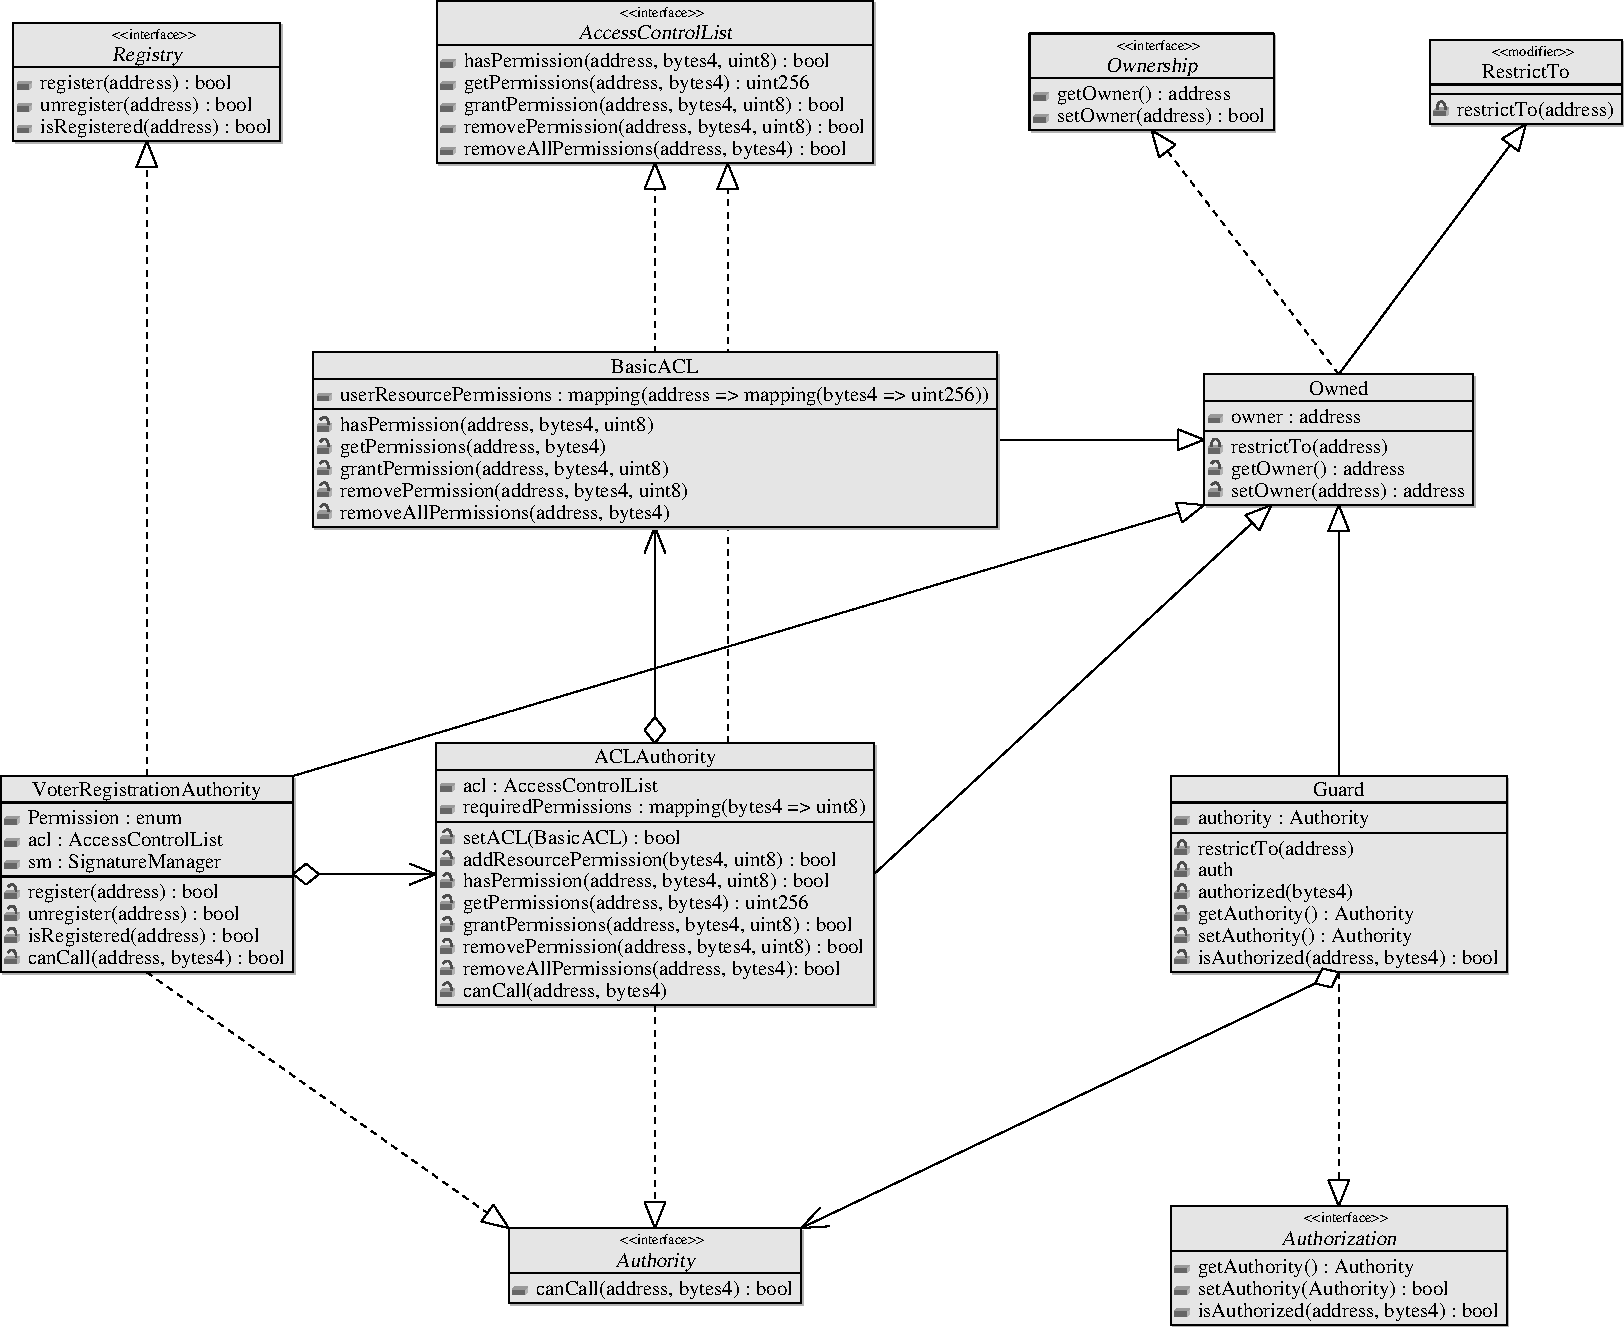
\includegraphics[width=\textwidth]{figures/authorization/figure}
  % \includestandalone[width=\textwidth]{\fig{authorization}}
\end{figure}

\subsubsection{Interface Registry}

The \solt{interface}, \sol{interface Registry}, introduces three \solt{function}
definitions required to achieve basic registry functionality:

\begin{enumerate}
  \item \sol{function register}, which \emph{registers} a \emph{subject}.

  \item \sol{function unregister}, which \emph{unregisters} a \emph{subject}.

  \item \sol{function isRegistered}, which evaluates whether a \emph{subject} is
    \emph{registered}.
\end{enumerate}

\begin{solidity}[interface Registry]
interface Registry {
  function register (address _subject) public returns (bool _success);
  function unregister (address _subject) public returns (bool _success);
  function isRegistered (address _subject) public constant returns (bool _isRegistered);
}
\end{solidity}

\begin{interface}
  \item \specification{}

  \begin{functions}
    \item \sol{function isRegistered (address _subject)}, evaluates whether some
      \emph{subject} is \emph{registered}.

      \begin{parameters}
        \item \sol{address _subject}, the \solt{address} of an account
          representing the \emph{subject}, to evaluate the \emph{registration}
          of.
      \end{parameters}

      \begin{returns}
        \item \sol{bool _isRegistered}, returns the \solt{true} if the
          \emph{subject} is \emph{registered}, otherwise \solt{false}.
      \end{returns}

    \item \sol{function unregister (address _subject)}, \emph{unregisters} a
      \emph{subject}.

      \begin{parameters}
        \item \sol{address _subject}, the account \solt{address} of the
          \emph{subject} who is to be \emph{unregistered}.
      \end{parameters}

      \begin{returns}
        \item \sol{bool _success}, resolves to \solt{true} if the operation was
          successful, otherwise \solt{false}.
      \end{returns}

    \item \sol{function register (address _subject)}, \emph{registers} a
      \emph{subject}.

      \begin{parameters}
        \item \sol{address _subject}, the account \solt{address} of the
          \emph{subject} who is to be \emph{registered}.
      \end{parameters}

      \begin{returns}
        \item \sol{bool _success}, resolves to \solt{true} if the operation was
          successful, otherwise \solt{false}.
      \end{returns}
  \end{functions}
\end{interface}


\subsubsection{Contract VoterRegistrationAuthority}

The \solt{contract}, \sol{contract VoterRegistrationAuthority}, is the final
component of our authorization design and is required to construct a generalized
voter registration authority capable of managing registered voters and
conducting elections.

% signatureMap['vote'] = bytes4(sha3('vote(uint8[],uint8[])'));
\begin{solidity}[contract VoterRegistrationAuthority]
contract VoterRegistrationAuthority is Owned, Registry, Authority {
  enum Permissions {
    Vote
  }

  AccessControlList acl;
  mapping (bytes32 => bytes4) resourceSignatures;

  constructor () public {
    acl = new ACLAuthority(true);

    resourceSignatures['vote'] = bytes4(sha3('vote()'));

    acl.setRequiredResourcePermission(
      resourceSignature('vote'),
      uint8(Permissions.Vote)
    );
  }

  function register (address _voter) public restrictTo(owner) returns (bool _success) {
    return acl.grantPermission(_voter, resourceSignatures['vote'], uint8(Permissions.Vote));
  }

  function unregister (address _voter) public restrictTo(owner) returns (bool _success) {
    return acl.revokePermission(_voter, resourceSignatures['vote'], uint8(Permissions.Vote));
  }

  function isRegistered (address _voter) public constant returns (bool _isRegistered) {
    return acl.hasPermission(_voter, resourceSignatures['vote'], uint8(Permissions.Vote));
  }

  function canCall (address _subject, bytes4 _resource) public constant returns (bool _canCall) {
    return acl.canCall(_subject, _resource);
  }
}
\end{solidity}

\todo{Finish documenting the VoterRegistrationAuthority implementation.}

\begin{state}
  \item \attributes

  \begin{public}
    \item \sol{AccessControlList acl} maintains the \solt{address} of an ACL
      implementation, a \solt{contract} which implements \sol{interface
      AccessControlList}.

    \item \sol{mapping (bytes32 => bytes4) resourceSignatures} maintains a
      mapping of strings, \sol{bytes32}, to \solt{function} signature,
      \sol{bytes4}.
  \end{public}
\end{state}

\begin{code}
  \item \operations

  \begin{constructor}
    \item \sol{constructor (bool _createACL)}, upon creation and initialization
      of this \solt{contract} the \solt{constructor} can deploy a
      \solt{contract}, \sol{contract BasicACL}, if the \solt{bool}, \sol{bool
      _createACL}, is set to \solt{true}.

      \begin{parameters}
      \item \sol{bool _createACL}, set to \solt{true} to deploy an ACL
        implementation, \sol{contract BasicACL}, in addition to this
        \solt{contract}; otherwise \solt{false}.
      \end{parameters}
  \end{constructor}

  \begin{functions}
    \item \sol{function setAcl (AccessControlList _acl)}, updates the
      \solt{contract} reference which is responsible for managing ACL requests.

      \begin{modifiers}
        \item \sol{modifier restrictTo (owner)}, restricts access to the
          \solt{function} such that \emph{only} the current \solt{owner} of the
          \sol{contract} can call it.
      \end{modifiers}

      \begin{parameters}
        \item \sol{AccessControlList _acl}, the ACL implementation which access
          control responsibilities are to be delegated to.
      \end{parameters}

      \begin{returns}
        \item \sol{bool _success}, resolves to \solt{true} if the operation was
          successful, otherwise \solt{false}.
      \end{returns}


    \item \sol{function setRequiredResourcePermission (bytes4 _resource, uint8 _permission)},
      updates the mapping representing the \emph{permission} required to access
      some \emph{resource}, \solt{function} signature.

      \begin{modifiers}
        \item \sol{modifier restrictTo (owner)}, restricts access to the
          \solt{function} such that \emph{only} the current \solt{owner} of the
          \sol{contract} can call it.
      \end{modifiers}

      \begin{parameters}
        \item \sol{bytes4 _resource}, the \emph{resource}, \solt{function}
          signature, which the \emph{permission} is to be modified for.

        \item \sol{uint8 _permission}, a \solt{uint8} value representing the
          \emph{permission-bit} required for the \emph{resource}.
      \end{parameters}

      \begin{returns}
        \item \sol{bool _success}, resolves to \solt{true} if the operation was
          successful, otherwise \solt{false}.
      \end{returns}


    \item \sol{function canCall (address _subject, bytes4 _resource)}, evaluates
      whether a \emph{subject} can access to some \emph{resource} by validating
      with the ACL implementation that the \emph{subject} has the required
      \emph{resource} \emph{permission}.

      \begin{parameters}
        \item \sol{address _subject}, the \emph{subject}, Ethereum account,
          whose \emph{permissions} are being evaluated.

        \item \sol{bytes4 _resource}, the \emph{resource}, \solt{contract
          function}, which the \emph{subject's} \emph{permissions} are being
          evaluated against.
      \end{parameters}

      \begin{returns}
        \item \sol{bool _canCall}, resolves to \solt{true} if the
          \emph{subject}, \sol{address _subject}, is permitted to access the
          \emph{resource}, \sol{bytes4 _resource}, otherwise \solt{false}.
      \end{returns}


    \item
      \sol{function hasPermission (address _subject, bytes4 _resource, uint8 _permission)}, \\
      \sol{function getPermissions (address _subject, bytes4 _resource)}, \\
      \sol{function setPermissions (address _subject, bytes4 _resource, uint256 _permissions)}, \\
      \sol{function grantPermission (address _subject, bytes4 _resource, uint8 _permission)}, \\
      \sol{function revokePermission (address _subject, bytes4 _resource, uint8 _permission)}, \\
      all ACL responsibilities originating from \sol{interface AccessControlList}
      are delegated to the provided ACL implementation stored in
      \sol{AccessControlList acl}.

      \begin{modifiers}
        \item \sol{modifier restrictTo (owner)}, restricts access to the
          \solt{function} such that \emph{only} the current \solt{owner} of the
          \solt{contract} can call this \solt{function}; this applies to
          \solt{function}[s] \sol{setPermissions}, \sol{grantPermission}, and
        \sol{revokePermission}.
      \end{modifiers}
  \end{functions}
\end{code}



% Section: Election Components
% \section{Election Components}

This section explores the components relating to elections; election contracts:

\begin{enumerate}
  \item \emph{First-Past-the-Post},
  \item \emph{Range Vote}, and
  \item \emph{Single Transferable Vote}.
\end{enumerate}

% \begin{figure}[H]
%   \centering
%   \caption{Authorization dependency graph modeling.}% \label{fig:authorization}
%   \figurepdf[width=\textwidth]{authorization}
%   % 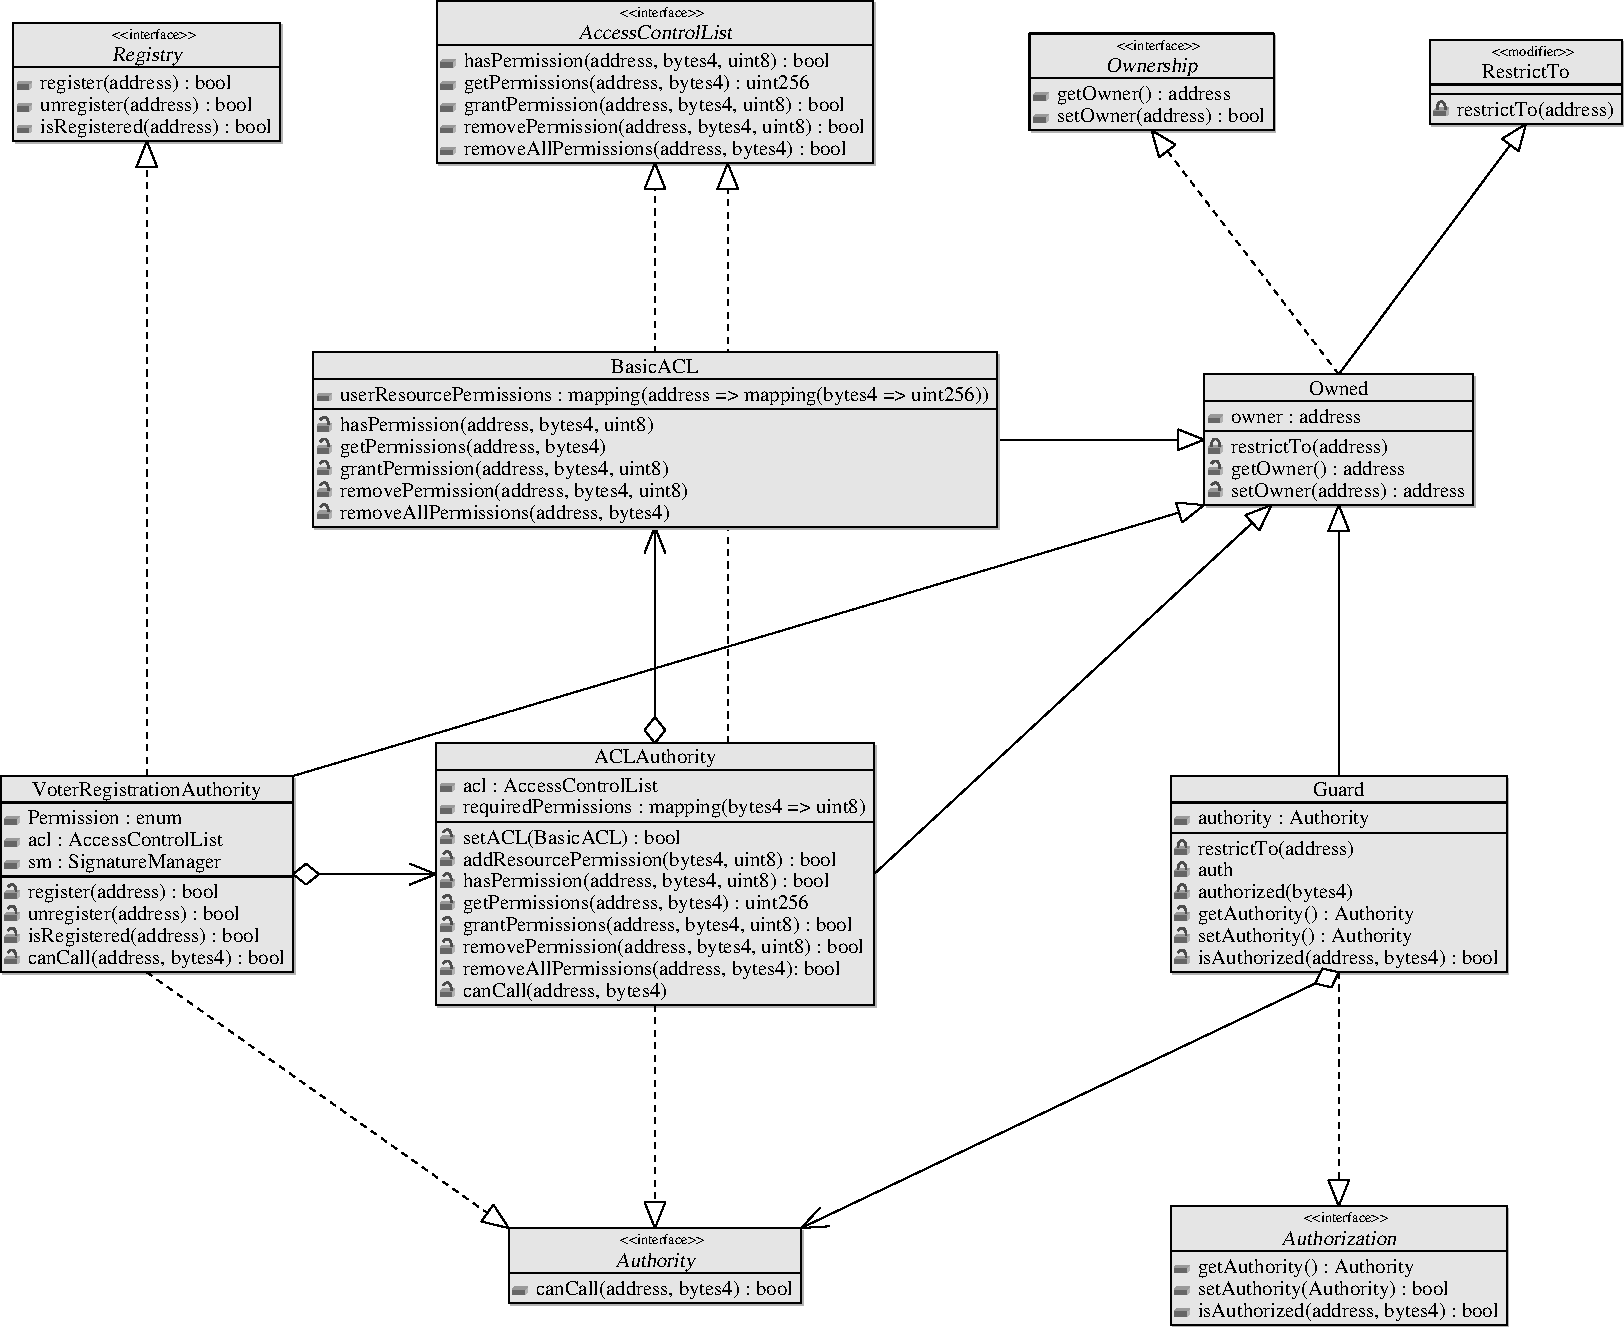
\includegraphics[width=\textwidth]{figures/authorization/figure}
%   % \includestandalone[width=\textwidth]{\fig{authorization}}
% \end{figure}

% \subsection{Finite State Machine}

% \subsection{First-Past-the-Post}
% The first-past-the-post \solt{contract} is the simplest election \solt{contract}
% implementation.

\subsection{Election Contracts}

\subsubsection{Contract FirstPastThePost}

The first-past-the-post \solt{contract} is the simplest election \solt{contract}
implementation.

\begin{solidity}[contract FirstPastThePost]
contract FirstPastThePost is Owned, Guard {
  uint public creationTime = now;

  Choice[] public choices;
  mapping(address => bool) public voted;
  Choice public winner;

  enum Phase { Configuration, Frozen, Vote, Tally }

  struct PhaseProperties {
    Phase phase;
    uint startTime;
    uint endTime;
    Phase nextPhase;
  }

  mapping (Phase => PhaseProperties) phases;
  Phase public phase = Phase.Configuration;

  constructor () {
    phases[Phase.Configuration] = PhaseProperties({
      phase: Phase.Configuration,
      start_time: now,
      end_time: 0,
      next_phase: Phase.Configuration
    });
  }

  // This is the current phase.
  uint public freezeTime;

  // Start and end time for the election.
  uint public voteStartTime;
  uint public voteEndTime;

  // This is a type for a single proposal.
  struct Choice {
    // Short name (up to 32 bytes).
    bytes32 name;

    // TODO: choice description?
    // bytes32 description;

    // Number of accumulated votes.
    uint40 voteCount;
  }

  // Restrict calls to _account.
  modifier restrictTo(address _account) {
    require(msg.sender == _account);
    _;
  }

  // Check current stage.
  modifier atPhase(Phase _phase) {
    require(phase == _phase);
    _;
  }

  // This modifier goes to the next phase after the function is done.
  modifier transitionNextPhase() {
    _;
    nextPhase();
  }

  // Move into next phase.
  function nextPhase() internal {
    phase = Phase(uint(phase) + 1);
  }

  // Perform timed transitions. Be sure to mention this modifier first,
  // otherwise the guards will not take the new stage into account.
  modifier timedTransitions() {
    if (phase == Phase.Frozen && now >= voteStartTime)
      nextPhase();
    if (phase == Phase.Vote && now >= voteEndTime)
      nextPhase();
    // The other stages transition by transaction
    _;
  }

  /* Election Functions */
  // Freeze the configuration.
  function freeze() restrictTo(owner) atPhase(Phase.Configuration) transitionNextPhase {
    require(voteStartTime > now);
    require(choices.length > 1);
    freezeTime = now;
    delete owner;
  }

  // Cast a ballot.
  function vote(uint8 choice) timedTransitions atPhase(Phase.Vote) {
    // Each address can only vote once.
    require(!voted[msg.sender]);
    voted[msg.sender] = true;

    choices[choice].voteCount += 1;
  }

  // Tally ballots.
  function tally() timedTransitions atPhase(Phase.Tally) {
    winner = choices[0];
    for (uint8 i = 0; i < choices.length; i++) {
      if (choices[i].voteCount > winner.voteCount)
        winner = choices[i];
    }
  }

  /* Configuration Functions */
  constructor () {}

  function setVoteStartTime(uint _voteStartTime) atPhase(Phase.Configuration) restrictTo(owner) {
    voteStartTime = _voteStartTime;
  }

  function setVoteEndTime(uint _voteEndTime) atPhase(Phase.Configuration) restrictTo(owner) {
    voteEndTime = _voteEndTime;
  }

  function addChoices(bytes32[] _choices) atPhase(Phase.Configuration) restrictTo(owner) {
    for (uint i = 0; i < _choices.length; i++) {
      choices.push(Choice({
        name: _choices[i],
        voteCount: 0
      }));
    }
  }

  function addChoice(bytes32 _name) atPhase(Phase.Configuration) restrictTo(owner) {
    choices.push(Choice({
      name: _name,
      voteCount: 0
    }));
  }

  //   function modifyChoice(uint8 key, bytes32 _name)
  //     atPhase(Phase.Configuration)
  //     restrictTo(owner)
  //   {
  //     require(key < choices.length-1);
  //
  //     choices[key] = Choice({
  //       name: _name,
  //       voteCount: 0
  //     });
  //   }
}
\end{solidity}

\begin{state}
  \item \attributes

  \begin{public}
    \item \sol{AccessControlList choices} maintains the \solt{address} of an ACL
      implementation, a \solt{contract} which implements \sol{interface
      AccessControlList}.

    \item \sol{mapping (bytes4 => uint8) requiredResourcePermissions} maintains a
      mapping of \solt{function}[s], \sol{bytes4}, to required
      \emph{permission}, \sol{uint8}.
  \end{public}
\end{state}

\begin{code}
  \item \operations

  \begin{constructor}
    \item \sol{constructor (bool _createACL)}, upon creation and initialization
      of this \solt{contract} the \solt{constructor} can deploy a
      \solt{contract}, \sol{contract BasicACL}, if the \solt{bool}, \sol{bool
      _createACL}, is set to \solt{true}.

      \begin{parameters}
      \item \sol{bool _createACL}, set to \solt{true} to deploy an ACL
        implementation, \sol{contract BasicACL}, in addition to this
        \solt{contract}; otherwise \solt{false}.
      \end{parameters}
  \end{constructor}

  \begin{functions}
    \item \sol{function setAcl (AccessControlList _acl)}, updates the
      \solt{contract} reference which is responsible for managing ACL requests.

      \begin{modifiers}
        \item \sol{modifier restrictTo (owner)}, restricts access to the
          \solt{function} such that \emph{only} the current \solt{owner} of the
          \sol{contract} can call it.
      \end{modifiers}

      \begin{parameters}
        \item \sol{AccessControlList _acl}, the ACL implementation which access
          control responsibilities are to be delegated to.
      \end{parameters}

      \begin{returns}
        \item \sol{bool _success}, resolves to \solt{true} if the operation was
          successful, otherwise \solt{false}.
      \end{returns}


    \item \sol{function setRequiredResourcePermission (bytes4 _resource, uint8 _permission)},
      updates the mapping representing the \emph{permission} required to access
      some \emph{resource}, \solt{function} signature.

      \begin{modifiers}
        \item \sol{modifier restrictTo (owner)}, restricts access to the
          \solt{function} such that \emph{only} the current \solt{owner} of the
          \sol{contract} can call it.
      \end{modifiers}

      \begin{parameters}
        \item \sol{bytes4 _resource}, the \emph{resource}, \solt{function}
          signature, which the \emph{permission} is to be modified for.

        \item \sol{uint8 _permission}, a \solt{uint8} value representing the
          \emph{permission-bit} required for the \emph{resource}.
      \end{parameters}

      \begin{returns}
        \item \sol{bool _success}, resolves to \solt{true} if the operation was
          successful, otherwise \solt{false}.
      \end{returns}


    \item \sol{function canCall (address _subject, bytes4 _resource)}, evaluates
      whether a \emph{subject} can access to some \emph{resource} by validating
      with the ACL implementation that the \emph{subject} has the required
      \emph{resource} \emph{permission}.

      \begin{parameters}
        \item \sol{address _subject}, the \emph{subject}, Ethereum account,
          whose \emph{permissions} are being evaluated.

        \item \sol{bytes4 _resource}, the \emph{resource}, \solt{contract
          function}, which the \emph{subject's} \emph{permissions} are being
          evaluated against.
      \end{parameters}

      \begin{returns}
        \item \sol{bool _canCall}, resolves to \solt{true} if the
          \emph{subject}, \sol{address _subject}, is permitted to access the
          \emph{resource}, \sol{bytes4 _resource}, otherwise \solt{false}.
      \end{returns}


    \item
      \sol{function hasPermission (address _subject, bytes4 _resource, uint8 _permission)}, \\
      \sol{function getPermissions (address _subject, bytes4 _resource)}, \\
      \sol{function setPermissions (address _subject, bytes4 _resource, uint256 _permissions)}, \\
      \sol{function grantPermission (address _subject, bytes4 _resource, uint8 _permission)}, \\
      \sol{function revokePermission (address _subject, bytes4 _resource, uint8 _permission)}, \\
      all ACL responsibilities originating from \sol{interface AccessControlList}
      are delegated to the provided ACL implementation stored in
      \sol{AccessControlList acl}.

      \begin{modifiers}
        \item \sol{modifier restrictTo (owner)}, restricts access to the
          \solt{function} such that \emph{only} the current \solt{owner} of the
          \solt{contract} can call this \solt{function}; this applies to
          \solt{function}[s] \sol{setPermissions}, \sol{grantPermission}, and
        \sol{revokePermission}.
      \end{modifiers}
  \end{functions}
\end{code}


\subsubsection{Range Vote}

\subsubsection{Single Transferable Vote}


% Section: Delegation Components
% \section{Delegation Components}

This section explores the components relating to vote delegation. The delegation
components are responsible for managing the delegation of voters' votes to
delegates.

% \begin{figure}[H]
%   \centering
%   \caption{Authorization dependency graph modeling.}% \label{fig:authorization}
%   \figurepdf[width=\textwidth]{authorization}
%   % 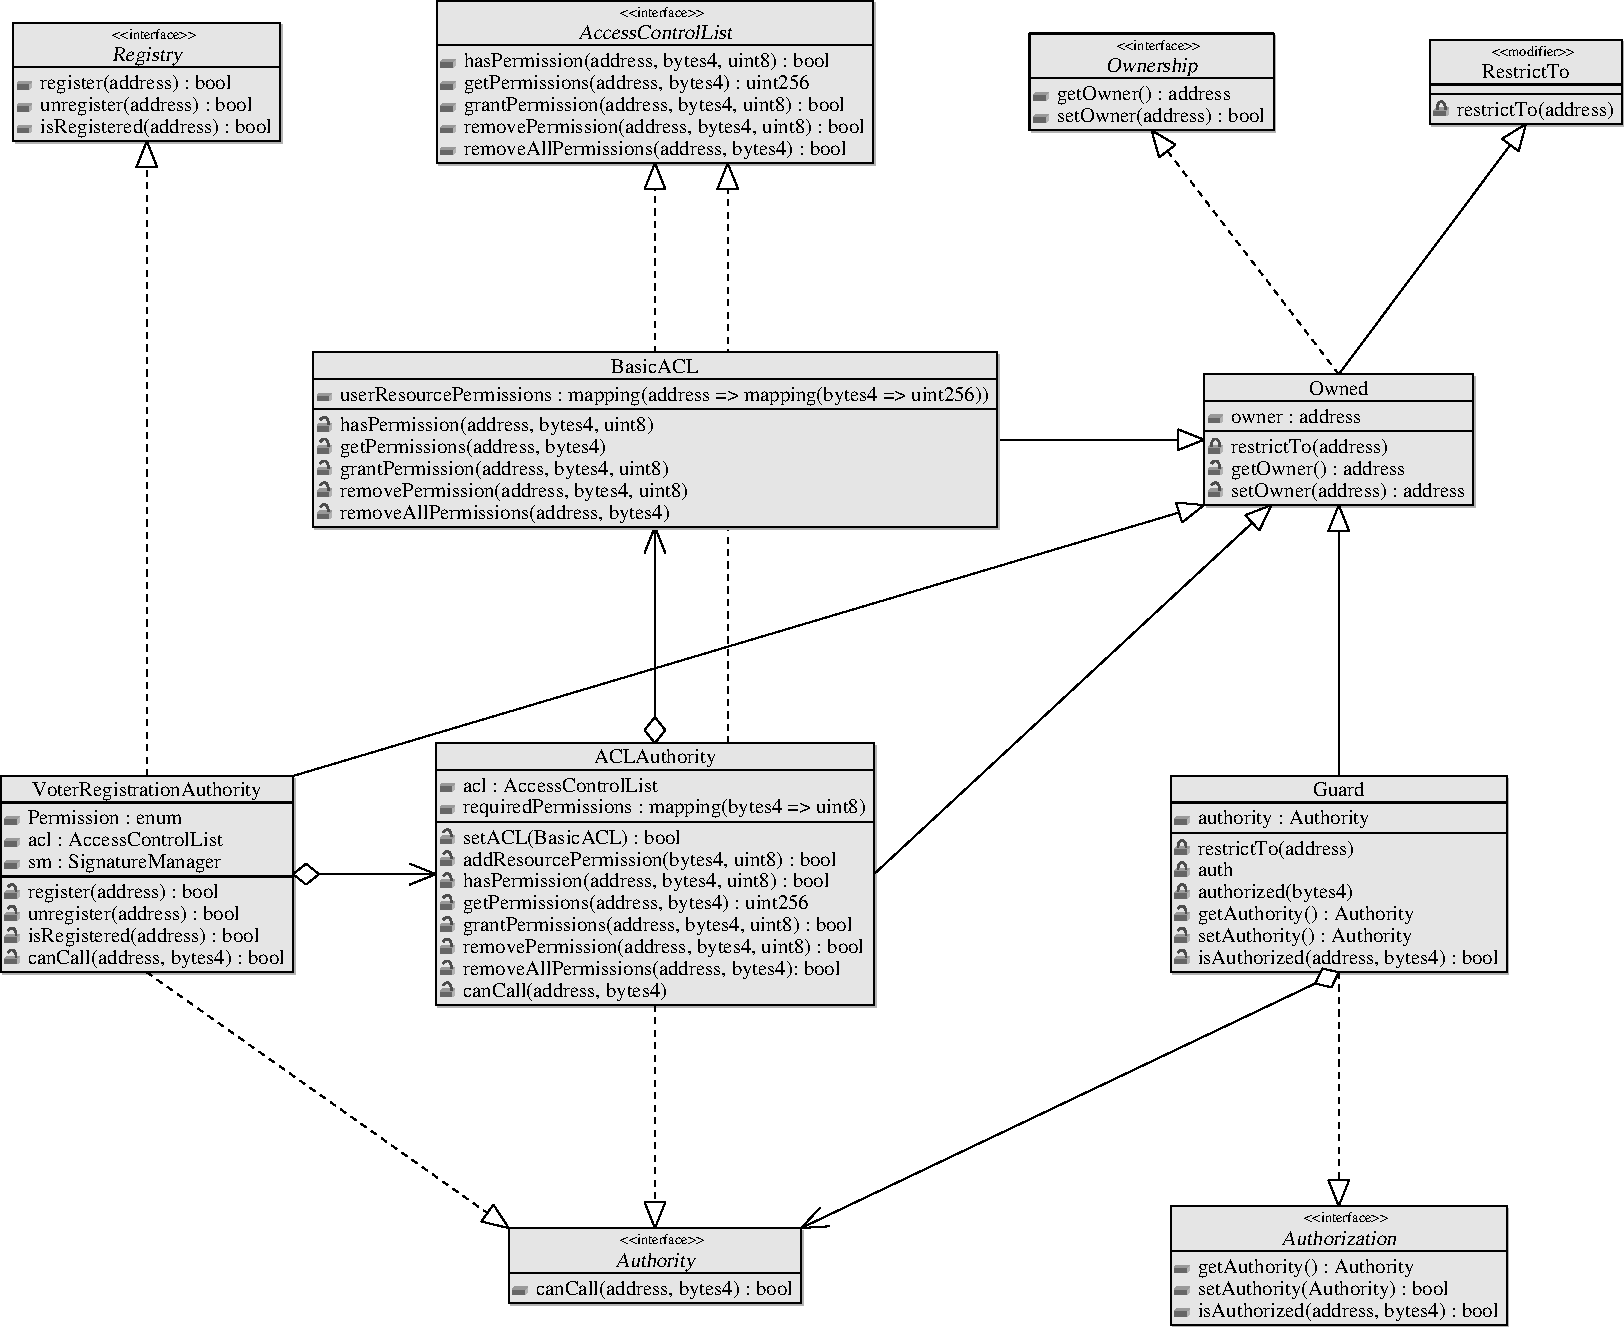
\includegraphics[width=\textwidth]{figures/authorization/figure}
%   % \includestandalone[width=\textwidth]{\fig{authorization}}
% \end{figure}

% Section: delegation
\subsection{Delegation Contracts}

\begin{solidity}[Vote Delegation]
mapping (address => Voter) voters;

function delegateVote (address delegate) public auth returns (bool _success) {
  // The `auth` modifier prevents this function from being
  // called until the Authority has confirmed that the
  // the message sender has the proper privileges.
  Voter cursor;
  uint40 weight = voters[msg.sender].weight;

  // Cycle Detection
  mapping (address => bool) visited;
  visited[msg.sender] = true;
  visited[delegate] = true;

  cursor = voters[delegate];
  while (cursor.delegate) {
    address newDelegate = cursor.delegate;
    if (visited[newDelegate]) return false;
    cursor = voters[newDelegate];
    visited[newDelegate] = true;
  }

  // Decrement weights of old delegate chain.
  cursor = voters[msg.sender];
  while (cursor.delegate) {
    address newDelegate = cursor.delegate;
    cursor = voters[newDelegate];
    cursor.weight -= weight;
  }

  // Increment weights of new delegate chain.
  cursor = voters[msg.sender];
  cursor.delegate = delegate;
  while (cursor.delegate) {
    address newDelegate = cursor.delegate;
    cursor = voters[newDelegate];
    cursor.weight += weight;
  }

  return true;
}
\end{solidity}



